% !TeX spellcheck = es_MX
\documentclass[12pt, a4paper, titlepage]{article}
\usepackage[spanish]{babel}
\usepackage[utf8]{inputenc}
\usepackage[linesnumbered,lined,boxed,commentsnumbered]{algorithm2e}
\usepackage{enumitem,kantlipsum}
\usepackage{array}
\usepackage{placeins}
% Códigos y codificación para caracteres en español
\usepackage{listings}
\usepackage{color}
\lstset{literate=
	{á}{{\'a}}1 {é}{{\'e}}1 {í}{{\'i}}1 {ó}{{\'o}}1 {ú}{{\'u}}1
	{Á}{{\'A}}1 {É}{{\'E}}1 {Í}{{\'I}}1 {Ó}{{\'O}}1 {Ú}{{\'U}}1
	{à}{{\`a}}1 {è}{{\`e}}1 {ì}{{\`i}}1 {ò}{{\`o}}1 {ù}{{\`u}}1
	{À}{{\`A}}1 {È}{{\'E}}1 {Ì}{{\`I}}1 {Ò}{{\`O}}1 {Ù}{{\`U}}1
	{ä}{{\"a}}1 {ë}{{\"e}}1 {ï}{{\"i}}1 {ö}{{\"o}}1 {ü}{{\"u}}1
	{Ä}{{\"A}}1 {Ë}{{\"E}}1 {Ï}{{\"I}}1 {Ö}{{\"O}}1 {Ü}{{\"U}}1
	{â}{{\^a}}1 {ê}{{\^e}}1 {î}{{\^i}}1 {ô}{{\^o}}1 {û}{{\^u}}1
	{Â}{{\^A}}1 {Ê}{{\^E}}1 {Î}{{\^I}}1 {Ô}{{\^O}}1 {Û}{{\^U}}1
	{œ}{{\oe}}1 {Œ}{{\OE}}1 {æ}{{\ae}}1 {Æ}{{\AE}}1 {ß}{{\ss}}1
	{ű}{{\H{u}}}1 {Ű}{{\H{U}}}1 {ő}{{\H{o}}}1 {Ő}{{\H{O}}}1
	{ç}{{\c c}}1 {Ç}{{\c C}}1 {ø}{{\o}}1 {å}{{\r a}}1 {Å}{{\r A}}1
	{€}{{\EUR}}1 {£}{{\pounds}}1
}
%%Appendix
\usepackage[toc,page]{appendix}

%%Tablas
\usepackage{tabularx}

%%otros
\usepackage{float}
\usepackage{subfig}
\usepackage{comment}

% http://ctan.org/pkg/booktabs
\usepackage{booktabs}
\newcommand{\tabitem}{~~\llap{\textbullet}~~}

%%Imágenes
\usepackage{graphicx}

%%Colores de texto 
\usepackage{xcolor}
\usepackage{colortbl}

%%Links
\usepackage[hidelinks]{hyperref}

%%Comentarios
\usepackage{verbatim}

%%PARA IMÁGENES EN LÍNEA
%\usepackage[english]{babel}

%%Acrónimos
\usepackage[acronym]{glossaries}

%%Glosario
\usepackage{glossaries}

\usepackage{pdfpages}

%%ESTILO DE CÓDIGO
\lstdefinestyle{codeStyle}{
	backgroundcolor=\color{backcolour}, commentstyle=\color{commentcolor},
	keywordstyle=\color{guindapoli},
	numberstyle=\tiny\color{azulescom},
	stringstyle=\color{azulfuerte},
	basicstyle=\ttfamily\footnotesize,
	breakatwhitespace=false, 
	breaklines=true, 
	captionpos=b,
	keepspaces=true,
	numbers=left,
	numbersep=5pt,
	showspaces=false,
	showstringspaces=false,
	showtabs=false,
	tabsize=3
}
\definecolor{delim}{RGB}{20,105,176}

%% JSON
\lstdefinelanguage{json}{
	basicstyle=\normalfont\ttfamily,
	numbers=left,
	numberstyle=\tiny\color{azulescom},
	stringstyle=\color{azulfuerte},
	stepnumber=1,
	numbersep=8pt,
	showstringspaces=false,
	breaklines=true,
	backgroundcolor=\color{backcolour},
	literate=
	*{0}{{{\color{azulfuerte}0}}}{1}
	{1}{{{\color{azulfuerte}1}}}{1}
	{2}{{{\color{azulfuerte}2}}}{1}
	{3}{{{\color{azulfuerte}3}}}{1}
	{4}{{{\color{azulfuerte}4}}}{1}
	{5}{{{\color{azulfuerte}5}}}{1}
	{6}{{{\color{azulfuerte}6}}}{1}
	{7}{{{\color{azulfuerte}7}}}{1}
	{8}{{{\color{azulfuerte}8}}}{1}
	{9}{{{\color{azulfuerte}9}}}{1}
	{:}{{{\color{guindapoli}{:}}}}{1}
	{,}{{{\color{guindapoli}{,}}}}{1}
	{\{}{{{\color{guindapoli}{\{}}}}{1}
	{\}}{{{\color{guindapoli}{\}}}}}{1}
	{[}{{{\color{guindapoli}{[}}}}{1}
	{]}{{{\color{guindapoli}{]}}}}{1},
}

\lstset{style=codeStyle}


\definecolor{lightgray}{rgb}{.9,.9,.9}
\definecolor{darkgray}{rgb}{.4,.4,.4}
\definecolor{purple}{rgb}{0.65, 0.12, 0.82}

%% Javascript
\lstdefinelanguage{JavaScript}{
	keywords={typeof, new, true, false, catch, function, return, null, catch, switch, var, if, in, while, do, else, case, break, let, continue},
	keywordstyle=\color{blue}\bfseries,
	ndkeywords={class, export, boolean, throw, implements, import, this},
	ndkeywordstyle=\color{darkgray}\bfseries,
	identifierstyle=\color{black},
	sensitive=false,
	comment=[l]{//},
	morecomment=[s]{/*}{*/},
	commentstyle=\color{purple}\ttfamily,
	stringstyle=\color{red}\ttfamily,
	morestring=[b]',
	morestring=[b]"
}

\lstset{
	language=JavaScript,
	backgroundcolor=\color{lightgray},
	extendedchars=true,
	basicstyle=\footnotesize\ttfamily,
	showstringspaces=false,
	showspaces=false,
	numbers=left,
	numberstyle=\footnotesize,
	numbersep=9pt,
	tabsize=2,
	breaklines=true,
	showtabs=false,
	captionpos=b
}
%% ESTO ES PYTHON

\definecolor{maroon}{cmyk}{0, 0.87, 0.68, 0.32}
\definecolor{halfgray}{gray}{0.55}
\definecolor{ipython_frame}{RGB}{207, 207, 207}
\definecolor{ipython_bg}{RGB}{247, 247, 247}
\definecolor{ipython_red}{RGB}{186, 33, 33}
\definecolor{ipython_green}{RGB}{0, 128, 0}
\definecolor{ipython_cyan}{RGB}{64, 128, 128}
\definecolor{ipython_purple}{RGB}{170, 34, 255}

\lstset{
	breaklines=true,
	extendedchars=true,
	literate=
	{á}{{\'a}}1 {é}{{\'e}}1 {í}{{\'i}}1 {ó}{{\'o}}1 {ú}{{\'u}}1
	{Á}{{\'A}}1 {É}{{\'E}}1 {Í}{{\'I}}1 {Ó}{{\'O}}1 {Ú}{{\'U}}1
	{à}{{\`a}}1 {è}{{\`e}}1 {ì}{{\`i}}1 {ò}{{\`o}}1 {ù}{{\`u}}1
	{À}{{\`A}}1 {È}{{\'E}}1 {Ì}{{\`I}}1 {Ò}{{\`O}}1 {Ù}{{\`U}}1
	{ä}{{\"a}}1 {ë}{{\"e}}1 {ï}{{\"i}}1 {ö}{{\"o}}1 {ü}{{\"u}}1
	{Ä}{{\"A}}1 {Ë}{{\"E}}1 {Ï}{{\"I}}1 {Ö}{{\"O}}1 {Ü}{{\"U}}1
	{â}{{\^a}}1 {ê}{{\^e}}1 {î}{{\^i}}1 {ô}{{\^o}}1 {û}{{\^u}}1
	{Â}{{\^A}}1 {Ê}{{\^E}}1 {Î}{{\^I}}1 {Ô}{{\^O}}1 {Û}{{\^U}}1
	{œ}{{\oe}}1 {Œ}{{\OE}}1 {æ}{{\ae}}1 {Æ}{{\AE}}1 {ß}{{\ss}}1
	{ç}{{\c c}}1 {Ç}{{\c C}}1 {ø}{{\o}}1 {å}{{\r a}}1 {Å}{{\r A}}1
	{€}{{\EUR}}1 {£}{{\pounds}}1
}

\lstdefinelanguage{python}{
	morekeywords={access,and,break,class,continue,def,del,elif,else,except,exec,finally,for,from,global,if,import,in,is,lambda,not,or,pass,print,raise,return,try,while},
	morekeywords=[2]{abs,all,any,basestring,bin,bool,bytearray,callable,chr,classmethod,cmp,compile,complex,delattr,dict,dir,divmod,enumerate,eval,execfile,file,filter,float,format,frozenset,getattr,globals,hasattr,hash,help,hex,id,input,int,isinstance,issubclass,iter,len,list,locals,long,map,max,memoryview,min,next,object,oct,open,ord,pow,property,range,raw_input,reduce,reload,repr,reversed,round,set,setattr,slice,sorted,staticmethod,str,sum,super,tuple,type,unichr,unicode,vars,xrange,zip,apply,buffer,coerce,intern},
	sensitive=true,
	morecomment=[l]\#,
	morestring=[b]',
	morestring=[b]",
	morestring=[s]{'''}{'''},
	morestring=[s]{"""}{"""},
	morestring=[s]{r'}{'},
	morestring=[s]{r"}{"},
	morestring=[s]{r'''}{'''},
	morestring=[s]{r"""}{"""},
	morestring=[s]{u'}{'},
	morestring=[s]{u"}{"},
	morestring=[s]{u'''}{'''},
	morestring=[s]{u"""}{"""},
	% {replace}{replacement}{lenght of replace}
	% *{-}{-}{1} will not replace in comments and so on
	literate=
	{á}{{\'a}}1 {é}{{\'e}}1 {í}{{\'i}}1 {ó}{{\'o}}1 {ú}{{\'u}}1
	{Á}{{\'A}}1 {É}{{\'E}}1 {Í}{{\'I}}1 {Ó}{{\'O}}1 {Ú}{{\'U}}1
	{à}{{\`a}}1 {è}{{\`e}}1 {ì}{{\`i}}1 {ò}{{\`o}}1 {ù}{{\`u}}1
	{À}{{\`A}}1 {È}{{\'E}}1 {Ì}{{\`I}}1 {Ò}{{\`O}}1 {Ù}{{\`U}}1
	{ä}{{\"a}}1 {ë}{{\"e}}1 {ï}{{\"i}}1 {ö}{{\"o}}1 {ü}{{\"u}}1
	{Ä}{{\"A}}1 {Ë}{{\"E}}1 {Ï}{{\"I}}1 {Ö}{{\"O}}1 {Ü}{{\"U}}1
	{â}{{\^a}}1 {ê}{{\^e}}1 {î}{{\^i}}1 {ô}{{\^o}}1 {û}{{\^u}}1
	{Â}{{\^A}}1 {Ê}{{\^E}}1 {Î}{{\^I}}1 {Ô}{{\^O}}1 {Û}{{\^U}}1
	{œ}{{\oe}}1 {Œ}{{\OE}}1 {æ}{{\ae}}1 {Æ}{{\AE}}1 {ß}{{\ss}}1
	{ç}{{\c c}}1 {Ç}{{\c C}}1 {ø}{{\o}}1 {å}{{\r a}}1 {Å}{{\r A}}1
	{€}{{\EUR}}1 {£}{{\pounds}}1
	%
	{^}{{{\color{ipython_purple}\^{}}}}1
	{=}{{{\color{ipython_purple}=}}}1
	%
	{+}{{{\color{ipython_purple}+}}}1
	{*}{{{\color{ipython_purple}$^\ast$}}}1
	{/}{{{\color{ipython_purple}/}}}1
	%
	{+=}{{{+=}}}1
	{-=}{{{-=}}}1
	{*=}{{{$^\ast$=}}}1
	{/=}{{{/=}}}1,
	literate=
	*{-}{{{\color{ipython_purple}-}}}1
	{?}{{{\color{ipython_purple}?}}}1,
	%
	identifierstyle=\color{black}\ttfamily,
	commentstyle=\color{ipython_cyan}\ttfamily,
	stringstyle=\color{ipython_red}\ttfamily,
	keepspaces=true,
	showspaces=false,
	showstringspaces=false,
	rulecolor=\color{ipython_frame},
	frame=single,
	frameround={t}{t}{t}{t},
	framexleftmargin=6mm,
	numbers=left,
	numberstyle=\tiny\color{halfgray},
	backgroundcolor=\color{ipython_bg},
	% extendedchars=true,
	basicstyle=\scriptsize,
	keywordstyle=\color{ipython_green}\ttfamily,
}
%------------------------------------------------ESTABLECER COLORES------------------------------------------------%

\definecolor{guindapoli}{RGB}{102, 0, 51}
\definecolor{azulescom}{RGB}{0, 0, 102}
\definecolor{azulclaro}{RGB}{222, 232, 255}
\definecolor{azulfuerte}{RGB}{60, 150, 250}

%------------------------------------------------COLORES PARA CÓDIGO------------------------------------------------%

\definecolor{commentcolor}{RGB}{ 192, 192, 192 }
\definecolor{backcolour}{RGB}{ 249, 249, 249 }

%------------------------------------------------FIN DE COLORES------------------------------------------------%

%------------------------------------------------ACRÓNIMOS------------------------------------------------%

\newacronym{mvc}{MVC}{Modelo-Vista-Controlador}
\newacronym{orm}{ORM}{Object Relational Manager}
\newacronym{wsgi}{WSGI}{Web Server Gateway Interface}
\newacronym{dbms}{DBMS}{Sistema de gestión de base de datos}
\newacronym{bert}{BERT}{Bidirectional Encoder Representations from Transformers}
\newacronym{pln}{PLN}{Procesamiento del Lenguaje Natural}
\newacronym{mlm}{MLM}{Modelado de Lenguaje Enmascarado}
\newacronym{gpt}{GPT}{Generative Pretrained Transformer}
\newacronym{bpe}{BPE}{Byte Pair Encoding}
\newacronym{wip}{WIP}{Work In Progress}
\newacronym{cls}{CLS}{Classification}
\newacronym{sep}{SEP}{Separate}
\newacronym{json}{JSON}{Javascript Object Notation}
\newacronym{url}{URL}{Uniform Source Locator}
\newacronym{http}{HTTP}{Hypertext Transfer Protocol}
\newacronym{tcp}{TCP}{Transmission Control Protocol}
\newacronym{udp}{UDP}{User Datagram Protocol}
\newacronym{imap}{IMAP}{Internet Message Access Protocol}
\newacronym{pop}{POP}{Post Office Protocol}
\newacronym{smtp}{SMTP}{Simple Mail Transfer Protocol}
\newacronym{vps}{VPS}{Virtual Private Server}
\newacronym{ssl}{SSL}{Secure Socket Layer}
\newacronym{fqdn}{FQDN}{Fully Qualified Domain Name}
\newacronym{aws}{AWS}{Amazon Web Services}
\newacronym{gpu}{GPU}{Graphic Processor Unit}
\newacronym{ec2}{EC2}{Elastic Compute Cloud}
\newacronym{ui}{UI}{User Interface}
\newacronym{api}{API}{Application Programm Interface}
\newacronym{gcp}{GCP}{Google Cloud Platform}
\newacronym{sdk}{SDK}{Software Development Kit}
\newacronym{html}{HTML}{Hypertext Markup Language}
\newacronym{css}{CSS}{Cascading Style Sheet}
\newacronym{ecma}{ECMA}{European Computer Manufacturers Association}
\newacronym{https}{HTTPS}{Hypertext Transfer Protocol Secure}
\newacronym{tls}{TLS}{Transport Layer Security}
\newacronym{sql}{SQL}{Structured Query Language}
\newacronym{cad}{CAD}{Computer Aided Design}
\newacronym{cli}{CLI}{Command Line Interface}
\newacronym{s3}{S3}{Simple Storage Service}
\newacronym{hdd}{HDD}{Hard Drive Disk}
\newacronym{ssd}{SSD}{Solid State Drive}
\newacronym{iso}{ISO}{International Standardization Organization}
\newacronym{xml}{XML}{Extensible Markup Language}
\newacronym{svg}{SVG}{Scalable Vector Graphics}
\newacronym{rnn}{RNN}{Recurrent Neural Network}
\newacronym{lstm}{LSTM}{Long Short Term Memory}
%------------------------------------------------FINAL DE ACRÓNIMOS------------------------------------------------%

\begin{document}
	%%PARA QUE DETECTE HASTA SUBSUBSECTION
	\setcounter{secnumdepth}{3}
	
	%%%%%%%%%%%%%%%%%%%%%%%%%%%%%%%%%%%%%%%%%%%%%%%%%%%%%%%%%
	%                                                       																																		  %
	%                                                      																																	  		  %
	%              																	PORTADA  																				  			 %
	%                                                      																																			  %
	%                                                      																																			  %
	%%%%%%%%%%%%%%%%%%%%%%%%%%%%%%%%%%%%%%%%%%%%%%%%%%%%%%%%%
	\begin{titlepage}	
		
		\newcommand{\HRule}{\rule{\linewidth}{0.5mm}}									%%%\left
		%%%
		\begin{minipage}{0.48\textwidth} \begin{flushleft}
				
\includegraphics[scale = 0.10]{Imagenes/Logos/logoescom.png}
		\end{flushleft}\end{minipage}
		\begin{minipage}{0.48\textwidth} \begin{flushright}
				
\includegraphics[scale = 0.55]{Imagenes/Logos/logoipn.png}
		\end{flushright}\end{minipage}
		
		%%%
		\vspace*{.25cm}								%%%
		
		\begin{center}
			
			\begin{LARGE}
				\textcolor{guindapoli}{INSTITUTO POLITÉCNICO NACIONAL}\\
			\end{LARGE}	
			
			\vspace*{0.2in}
			
			\begin{Large}
				\textcolor{azulescom}{ESCUELA SUPERIOR DE CÓMPUTO}\\
			\end{Large}	
			
			\vspace*{0.4in}
			
			\begin{large}
				Manual Técnico\\
			\end{large}	
			
			\vspace*{0.4in}
			
			\begin{large}
				Trabajo Terminal TT2020-B002\\
			\end{large}
			
			\vspace*{0.2in}
			
			\begin{Large}
				\textbf{Generador de versos musicales en el idioma
					inglés por medio de procesamiento de lenguaje
					natural y redes neuronales}\\
			\end{Large}
			
			\vspace*{0.2in}
			
			\rule{80mm}{.1mm}\\
			\vspace*{0.1in}
			
			\begin{large}
				\begin{center}
					\textbf{Presentan}:\\
					Espinosa de los Monteros Lechuga Jaime Daniel\\
					Nava Romo Edgar Adrián\\
					Salgado Gómez Alfredo Emilio\\
				\end{center}
			\end{large}
			
			\begin{large}
				\textbf{Directores}:\\
				Olga Kolesnikova\\
				Ariel López Rojas\\
			\end{large}
			
		\end{center}
		
	\end{titlepage}
	
	%%%%%%%%%%%%%%%%%%%%%%%%%%%%%%%%%%%%%%%%%%%%%%%%%%%%%%%%%
	%                                                       																																		  %
	%                                                      																																	  		  %
	%              																	 ÍNDICE  																				  			 	  %
	%                                                      																																			  %
	%                                                      																																			  %
	%%%%%%%%%%%%%%%%%%%%%%%%%%%%%%%%%%%%%%%%%%%%%%%%%%%%%%%%%
	% Firma directores
	\newpage
	\section*{Firmas de Directores}
	
	\vfill  % push the rest to the bottom of the page
	\noindent 
	\parbox[b]{0.4\linewidth}{% size of the first signature box
		\strut 
		Firmado por: \\[3cm]% This 2cm is the space for the signature under the names
		\hrule
		Profesor: Ariel López Rojas} 
	\hspace{1cm} % distance between the two signature blocks 
	\parbox[b]{0.4\linewidth}{% ...and the second one
		\strut 
		\\[3cm]% This 2cm is the space for the signature under the names
		\hrule
		Doctora Olga Kolesnikova} 
	\par\vspace{1cm} 
	\newpage
	% Rename Appendice to Anexos
	\renewcommand\appendixpagename{Índice}
	\renewcommand\appendixtocname{Índice}
	\appendixpageoff
	\begin{appendices}
		\renewcommand*\contentsname{{\textcolor{azulescom}{Índice.}}}
		\tableofcontents
		\newpage
		%%índice de figuras
		\renewcommand*\listfigurename{{\textcolor{azulescom}{Índice de figuras.}}}
		\listoffigures
		\newpage
		%%Índice de tablas
		\newpage
		\renewcommand*\listtablename{{\textcolor{azulescom}{Índice de cuadros.}}}
		\listoftables
		\newpage
	\end{appendices}
	
	\section{Presentación}
	El siguiente manual se ha desarrollado con la finalidad de dar a conocer la información necesaria para aquellos que darán soporte a la aplicación web, este les brindara información sobre los requerimientos, el desarrollo de la aplicación web, la generación del modelo, la conexión de la aplicación web con el modelo, las herramientas empleadas y la funcionalidad final.
	\section{Resumen}
	El manual detalla aspectos técnicos e informáticos relacionados con el desarrollo de la aplicación web, tiene como finalidad dar a conocer la información necesaria al personal que vaya a administrarlo, modificarlo o para realizar mantenimiento. En este manual se detallan las herramientas que se utilizaron durante el desarrollo. 
	\newpage
	\section{Introducción}
	Este manual describe los pasos necesarios para que cualquier persona con ciertas bases en sistemas computacionales pueda administrar, editar o configurar la aplicación web, y que cuando lo haga este responda de una manera adecuada.\\\\
	Se darán a conocer las herramientas que se utilizaron para el desarrollo de la aplicación web, su despliegue, así como se hará apoyo de diagramas e ilustraciones alusivas al funcionamiento del producto.	Además se detallarán los requerimientos mínimos de hardware y software para el correcto funcionamiento de la aplicación web.
	\section{Objetivo}
	Informar al usuario sobre la estructura y conformación de la aplicación web con el fin de que pueda darle soporte, realizar modificaciones o actualizaciones a la misma, a través de una descripción de los componentes y funcionalidades que lo conforman.
	\newpage
	\section{Requerimientos mínimos técnicos}
	\subsection{Requisitos de hardware de aplicaciones web}
	En la tabla siguiente se enumeran los requisitos
	de hardware mínimos y recomendados para la aplicación web.
	
	\begin{table}[!htbp]
		\caption[Requisitos hardware]{Requisitos de hardware mínimos y recomendados}
		\begin{tabular}{| p{4cm} | p{4cm} | p{4cm} |} 
			\hline
			\textbf{Componente} & \textbf{Mínimo} & \textbf{Recomendado} \\ 
			\hline
			Procesador & Procesador de x86 o x64 bits de doble núcleo de 1,9 gigahercios (GHz) o más con el conjunto de instrucciones SSE2 & Procesador de 64 bits de doble núcleo de 3,3 gigahercios (GHz) o más con el conjunto de instrucciones SSE2 \\ 
			\hline
			Memoria & 2 GB de RAM & 4 GB de RAM o más \\
			\hline
			Resolución  & Súper VGA con una resolución de 1024 x 768 & Súper VGA con una resolución de 1024 x 768 \\
			\hline
		\end{tabular}
	\end{table}
	
	
	La ejecución de aplicaciones basadas en modelo en un equipo
	que no cumpla los requisitos recomendados puede producir un
	rendimiento inadecuado. Además, puede experimentarse
	rendimiento satisfactorio ejecutando sistemas que usan otra
	configuración de hardware que los publicados aquí.\\\\
	Por ejemplo, un sistema con un procesador moderno
	de cuatro núcleos, velocidad de reloj más baja y más RAM.
	
	\subsection{Requisitos de red}
	Las aplicaciones basadas en modelo están diseñadas para funcionar
	mejor en redes que tienen los siguientes elementos:
	
	\begin{itemize}
		\item Ancho de banda superior a 50 KBps (400 kbps)
		\item Latencia inferior a 150 ms
	\end{itemize}
	
	Tenga en cuenta que estos valores son recomendaciones y no garantizan
	un rendimiento satisfactorio. Los valores recomendados se basan en los
	sistemas que usan solicitudes de un formulario con palabras usuales,
	el resultado podría variar.
	
	\section{Herramientas utilizadas para el desarrollo}
	\subsection{Python}
	Python es un lenguaje de programación orientado a objetos, de alto nivel con semántica dinámica. Sus estructuras de datos integradas de alto nivel, combinadas con el tipado y enlace dinámico, lo hacen muy atractivo para el desarrollo rápido de aplicaciones, así como para su uso en scripts o para conectar componentes ya existentes. La sintaxis simple y fácil de aprender de Python enfatiza la legibilidad y, por lo tanto, reduce el costo de mantenimiento del programa. Python admite módulos y paquetes, lo que fomenta la modularidad del programa y la reutilización del código. \cite{refQuesPython}
	\subsection{HTML}
	\acrfull{html} es un lenguaje de marcado que define la estructura de una página web y su contenido. \acrshort{html} consta de una serie de elementos que se utilizan para encerrar o envolver diferentes partes del contenido para que estos se visualicen o actúen de cierta manera. Las etiquetas adjuntas pueden hacer que una palabra o imagen sea un hipervínculo a otro lugar, pueden poner palabras en cursiva, hacer que la fuente sea más grande o pequeña, etc. \cite{refHtml} \\\\\
	\acrshort{html}5 es la versión más reciente de HTML, la cual integra nuevos elementos, atributos y comportamientos. Permite describir de mejor manera el contenido de la página web, así como mejora su conectividad con el servidor y almacenamiento, posibilita que las páginas web puedan operar sin conexión usando los datos almacenados localmente del lado del cliente, otorga un mejor soporte al contenido multimedia, así como una mejor integración a APIs y un mejor diseño usando \acrshort{css}3.	\cite{refHtml2}
	\subsection{CSS}
	\acrfull{css} es el lenguaje para describir la presentación de las páginas web, así como hacerlas más atractivas. Permite adaptar la presentación a diferentes tipos de dispositivos. \acrshort{css} es independiente de \acrshort{html} y puede ser empleado con cualquier otro lenguaje de marcado basado en \acrshort{xml} o \acrshort{svg}. Usando CSS se pueden controlar con precisión cómo se ven los elementos \acrshort{html} en el navegador, que presentará para las etiquetas de marcado el diseño que cada uno desee. La separación de \acrshort{html} de \acrshort{css} facilita el mantenimiento de los sitios, compartir las hojas de estilo entre páginas y adaptarlas a distintos ámbitos. \cite{refcss}\\\\
	Es un lenguaje basado en reglas: cada usuario define las reglas que especifican los grupos de estilos que van a aplicarse a elementos particulares o grupos de elementos de la página web.\\\\
	Antes de CSS, las etiquetas como fuente, color, estilo de fondo, alineación, borde y tamaño tenían que repetirse en cada elemento de una página web. Ahora con los CSS, podemos definir cómo se van a comportar las etiquetas, al ser guardado en un archivo por separado, esta misma configuración puede usarse en otra página web ahorrando tiempo diseñándola. Además de que CSS provee de mejor y más detallados atributos para cada etiqueta.
	\subsection{JavaScript}
	JavaScript es un lenguaje de programación o secuencias de comandos que permite implementar funciones complejas en las páginas web. Estos scripts pueden ser desarrollados en el mismo \acrshort{html} para que sean ejecutados automáticamente cuando se carga dicha páginas web, estos scripts se proporcionan y ejecutan como texto sin formato. No necesitan una preparación especial ni una compilación para ejecutarse. \cite{refjs}\\\\
	JavaScript puede ejecutarse no solo en un navegador, sino también en un servidor, o en cualquier dispositivo que tenga un programa especial llamado JavaScript engine, el cual permite interpretar y ejecutar los scripts.\\\\
	JavaScript permite crear contenido dinámico dentro de las páginas web, reaccionar ante algunas acciones realizadas por los usuarios como lo son los clics del ratón, el movimiento del puntero o el presionar cierta tecla, permite enviar peticiones al servidor, así como descargar y subir archivos, además es posible obtener y configurar cookies, mostrar mensajes o alertas al usuario.
	\subsection{Flask}
	Flask es un mini marco (framework) web, esto es, un módulo de Python el cual permite desarrollar aplicaciones web. No cuenta con un Manejador de Objetos Relacionales u \acrshort{orm} por sus siglas en inglés, pero si cuenta con características como el enrutamiento de \acrshort{url}S y un motor de plantillas. En general es un marco de aplicación web \acrshort{wsgi}.\\\\
	La \acrfull{wsgi} es una especificación que describe cómo se va a comunicar un servidor web con una aplicación web, y como se pueden llegar a enlazar distintas aplicaciones web para procesar una solicitud o una petición.
	\subsection{Gunicorn}
	Gunicorn, también conocido como unicornio verde “Green Unicorn”, es una de las muchas implementaciones de un \acrfull{wsgi} y se usa comúnmente para ejecutar aplicaciones web hechas con Python. Esta implemente la especificación \acrshort{wsgi} de frameworks como Django, Flask o Bottle.
	\subsection{Amazon EC2}	
	Amazon \acrfull{ec2} \cite{amazon_ec2} proporciona una infraestructura de tecnologías de información que se ejecuta en la nube y funciona como un centro de datos que se ejecuta en su propia sede. Es ideal para empresas que necesitan rendimiento, flexibilidad y potencia al mismo tiempo.\\\\
	Amazon \acrshort{ec2} es un servicio que permite alquilar un servidor o máquina virtual de forma remota para ejecutar aplicaciones.
	\begin{comment}	
	\subsection{Amazon SageMaker}
	Amazon SageMaker \cite{amazon_sagemaker} es un servicio que ayuda a científicos y desarrolladores a construir, entrenar e implementar de manera rápida y sencilla modelos de machine learning.\\\\
	Para construir el modelo, este servicio cuenta con algoritmos de machine learning más utilizados que vienen preinstalados. También está preconfigurado para que pueda ejecutar Apache MXNet y TensorFlow.\\\\
	Para el entrenamiento, con un solo clic en la consola de servicio, es fácil comenzar a entrenar su modelo. Amazon SageMaker se encarga de cada infraestructura y facilita la escalabilidad. lo que permite entrenar los modelos a escala de peta-bytes Si se desea acelerar y simplificar el proceso de entrenamiento, se puede ajustar automáticamente el modelo para obtener la mejor precisión.\\\\
	Para desplegar el modelo entrenado, se aloja en un clúster de escalado automático de Amazon \acrshort{ec2}.
	\end{comment}	
	\subsection{Amazon S3}
	Amazon \acrfull{s3} \cite{amazon_s3}, como su nombre lo indica, es un servicio web proporcionado por \acrfull{aws} que proporciona almacenamiento altamente escalable en la nube.
	\newpage
	\section{Diagramas de la aplicación web}
	\subsection{Diagrama de casos de uso}
	En el diagrama de casos de uso se detalla el papel que desempeña la aplicación web con el usuario y con el servidor.	
	\begin{figure}[H] 
		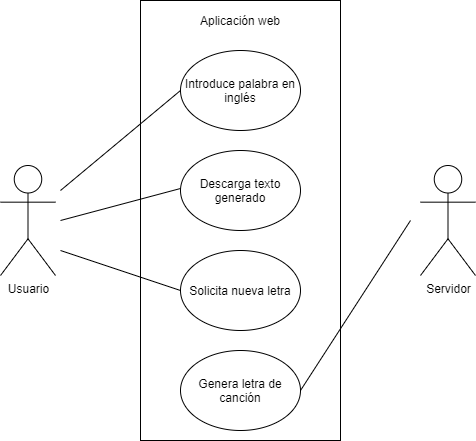
\includegraphics[width=13.5cm]{./Imagenes/Diagramas/CasoUso.png}
		\centering \caption{Diagrama de casos de uso}
	\end{figure}
	\newpage
	\begin{table}[hbt!]\caption{Caso de uso 1}% title of Table
		\centering % used for centering table
		\resizebox{13.5cm}{!} {
			\begin{tabular}{|c|c|}% centered columns (3 columns)
				\hline                        %inserts double horizontal lines
				\begin{tabular}[c]{@{}l@{}}Caso de uso\end{tabular}
				& \begin{tabular}[c]{@{}l@{}}Introduce palabra en inglés\end{tabular} \\% inserting body of the table 
				\hline				                     
				\begin{tabular}[c]{@{}l@{}}Actores\end{tabular}
				& \begin{tabular}[c]{@{}l@{}}Usuario\end{tabular} \\% inserting body of the table 
				\hline
				\begin{tabular}[c]{@{}l@{}}Descripción\end{tabular}
				& \begin{tabular}[c]{@{}l@{}}El usuario dentro de la aplicación web proporciona una palabra\\ en el idioma inglés para con ella poder generar un texto \end{tabular} \\
				\hline
			\end{tabular}\label{table:Caso de uso 1}% is used to refer this table in the text
		}
	\end{table}
	\begin{table}[hbt!]\caption{Caso de uso 2}% title of Table
		\centering % used for centering table
		\resizebox{13.5cm}{!} {
			\begin{tabular}{|c|c|}% centered columns (3 columns)
				\hline                        %inserts double horizontal lines
				\begin{tabular}[c]{@{}l@{}}Caso de uso\end{tabular}
				& \begin{tabular}[c]{@{}l@{}}Descargar texto generado\end{tabular} \\% inserting body of the table 
				\hline				                     
				\begin{tabular}[c]{@{}l@{}}Actores\end{tabular}
				& \begin{tabular}[c]{@{}l@{}}Usuario\end{tabular} \\% inserting body of the table 
				\hline
				\begin{tabular}[c]{@{}l@{}}Descripción\end{tabular}
				& \begin{tabular}[c]{@{}l@{}}El usuario dentro de la aplicación web tiene la posibilidad\\ de descargar el texto generado por el modelo  \end{tabular} \\
				\hline
			\end{tabular}\label{table:Caso de uso 2}% is used to refer this table in the text
		}
	\end{table}	
	\begin{table}[hbt!]\caption{Caso de uso 3}% title of Table
		\centering % used for centering table
		\resizebox{13.5cm}{!} {
			\begin{tabular}{|c|c|}% centered columns (3 columns)
				\hline                        %inserts double horizontal lines
				\begin{tabular}[c]{@{}l@{}}Caso de uso\end{tabular}
				& \begin{tabular}[c]{@{}l@{}}Solicitar nueva letra\end{tabular} \\% inserting body of the table 
				\hline				                     
				\begin{tabular}[c]{@{}l@{}}Actores\end{tabular}
				& \begin{tabular}[c]{@{}l@{}}Usuario\end{tabular} \\% inserting body of the table 
				\hline
				\begin{tabular}[c]{@{}l@{}}Descripción\end{tabular}
				& \begin{tabular}[c]{@{}l@{}}Al usuario dentro de la aplicación web se le da posibilidad de volver\\ a generar otra letra musical usando los mismos parámetros que proporcionó\\ o utilizando unos nuevos\end{tabular} \\
				\hline
			\end{tabular}\label{table:Caso de uso 3}% is used to refer this table in the text
		}
	\end{table}	
	\begin{table}[hbt!]\caption{Caso de uso 4}% title of Table
		\centering % used for centering table
		\resizebox{13.5cm}{!} {
			\begin{tabular}{|c|c|}% centered columns (3 columns)
				\hline                        %inserts double horizontal lines
				\begin{tabular}[c]{@{}l@{}}Caso de uso\end{tabular}
				& \begin{tabular}[c]{@{}l@{}}Genera letra de canción\end{tabular} \\% inserting body of the table 
				\hline				                     
				\begin{tabular}[c]{@{}l@{}}Actores\end{tabular}
				& \begin{tabular}[c]{@{}l@{}}Servidor\end{tabular} \\% inserting body of the table 
				\hline
				\begin{tabular}[c]{@{}l@{}}Descripción\end{tabular}
				& \begin{tabular}[c]{@{}l@{}}El servidor envia el texto generado por el modelo a la aplicación web,\\ la cual se encarga de mostrarla al usuario final \end{tabular} \\
				\hline
			\end{tabular}\label{table:Caso de uso41}% is used to refer this table in the text
		}
	\end{table}
	\newpage
	\section{Funcionamiento general del sistema}
	El siguiente diagrama muestra el funcionamiento general del producto, donde se ejemplifica a grandes rasgos la extracción del dataset con el cual, después de limpiarlo se realiza el entrenamiento del modelo, el cual puede generar textos, dichos textos en comunicación con el servidor web se muestran al usuario final.
	\begin{figure}[H] 
		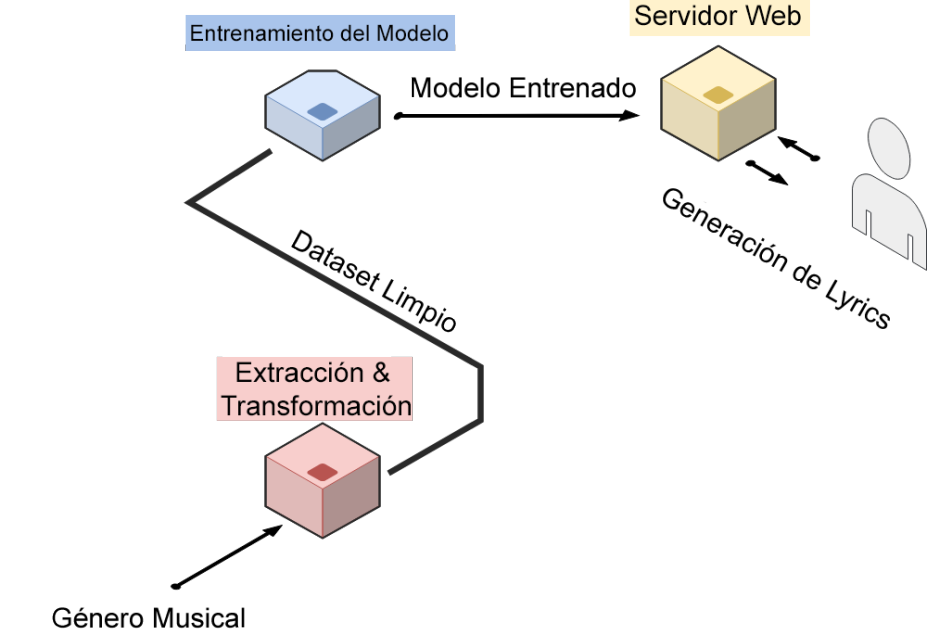
\includegraphics[width=13.5cm]{./Imagenes/Diagramas/general.png}
		\centering \caption{Diagrama general del sistema}
	\end{figure}
	\newpage
	\section{Base de datos}
	Lo primero que se realizo fue obtener una base de datos la cual contuviera en ella letras de canciones pertenecientes al género musical con el que íbamos a trabajar, que en este caso fue el género pop, así como que estas se encontraran en el idioma inglés. Para ello buscamos en distintas plataformas, datasets que cumplieran con estos requisitos y que estuvieran disponibles para su uso, es decir, de tipo open source.\\\\
	En Kaggle \cite{kaggle} se encontró un dataset llamado “Song lyrics for 6 musical genres” \cite{kaggleDataset} el cual contiene todos los datos necesarios para el sistema con un total de 160,790 letras de canciones con las tablas mostradas a continuación: 
	\begin{figure}[H]
		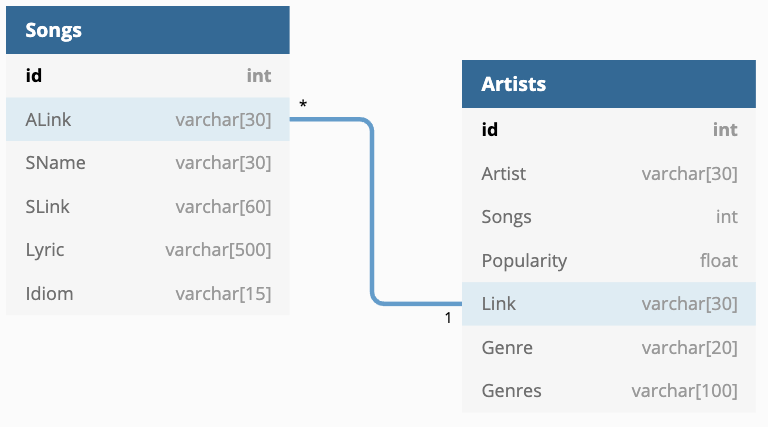
\includegraphics[width=12cm]{./Imagenes/BasedeDatos/diagrama_ER_BD.jpg}
		\centering 
		\caption{Diagrama entidad-relación de la base de datos}
	\end{figure}
	Dicha base de datos se obtuvo originalmente de la página de vagalume.com \cite{vagalume} e incluye 6 tipos de géneros musicales mencionados a continuación.
	\begin{itemize}
		\item Rock
		\item Pop
		\item Hip Hop
		\item Samba
		\item Sertanejo
		\item Funk Carioca
	\end{itemize}
	Como se puede observar, se tenía la columna “Genre” la cual fue utilizada para separar el dataset en géneros musicales y “Link” la cual servía como enlace a la segunda tabla. Se fusionaron tablas dando el siguiente resultado:
	\begin{figure}[H]
		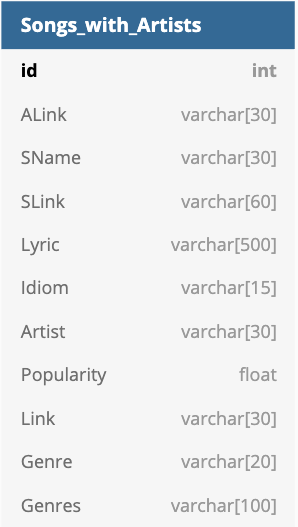
\includegraphics[width=5cm]{./Imagenes/BasedeDatos/Songs_with_Artists.png}
		\centering 
		\caption{Diagrama entidad-relación de la base de datos procesada}
	\end{figure}
	Posteriormente es necesario extraer la información precisa que se va utilizar para el entrenamiento del modelo, para ello se utilizaron las columnas de “Lyric” para seleccionar las letras que se utilizaran para entrenar el modelo, “Idiom” para separar las canciones en el idioma inglés y la columna de “Genre” para tamizar las canciones que forman parte del género pop, formando una base de datos simple la cual solo contiene las letras de canciones del género pop en el idioma inglés.
	\begin{figure}[H]
		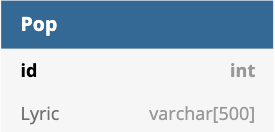
\includegraphics[width=5cm]{./Imagenes/BasedeDatos/Pop.png}
		\centering 
		\caption{Diagrama entidad-relación final}
	\end{figure}
	\newpage
	\section{Limpieza de la base de datos}
	Una vez obtenida la base de datos, es necesario hacer una inspección de esta misma para verificar que los estos datos sean útiles para proceder a generar un modelo, este paso resulta de suma importancia, ya que de esto depende que la precisión de los resultados del modelo.\\\\
	Para ello se identificarán datos que resulten incompletos, incorrectos, inexactos o no pertinentes para luego sustituirlos, modificarlos o en su caso, eliminar estos datos. \\\\\
	Estas inconsistencias en el conjunto de datos pueden ser causados por errores de entrada del usuario, corrupción de los datos, errores al realizar el scraping, o simplemente cuenta con caracteres que no nos interesa procesar. Una vez realizada esta limpieza, la base de datos será conciliable para usarse en el entrenamiento y así los resultados generados finales tendrán una mejor comprensión. \\\\
	Para ello se utilizó la librería de “Pandas” así como la librería de expresiones regulares. Para limpiar los datos se siguió el estándar de limpieza de datos: \cite{data_cleaning}
	\begin{enumerate}
		\item Remover caracteres innecesarios
		\item Eliminar Duplicados
		\item Evitar errores ortográficos de similitud
		\item Convertir los tipos de dato
		\item Tratar los valores nulos o faltantes
	\end{enumerate}
	Con la limpieza del conjunto de datos se tuvo como resultado una base de datos útil solo con los datos necesarios para poder tratarlos con el debido proceso para empezar el entrenamiento del modelo de la red neuronal, este proceso es necesario hacer solo una sola vez para cada género musical ingresado, en caso de que se lleguen a necesitar más datos, será necesario repetir el proceso para poder generar resultados de la manera más óptima posible. A continuación, se muestran las primeras líneas de la base de datos limpias.
	\begin{figure}[H]
		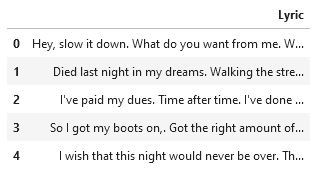
\includegraphics[width=7cm]{./Imagenes/BasedeDatos/ResultadosLimpiezaBasedeDatos.png}
		\centering 
		\caption{Resultados de limpieza en la base de batos}
	\end{figure}
	\newpage
	\section{Desarrollo del modelo}
	Para el desarrollo del modelo se utilizó una libreta de Kaggle. Cabe mencionar que el lenguaje de programación utilizado para el desarrollo del modelo fue Python, lo primero que se trabajó en la libreta, fue realizar la importación de librerías que se fueran a necesitar, las más importantes son:	
	\begin{itemize}
		\item Pandas: la cual nos permite manipular y analizar la información.
		\item Wordcloud: es una herramienta que nos ayuda al momento de generar la siguiente palabra de una oración.
		\item Tensorflow: una herramienta que nos ayuda en el procesamiento del aprendizaje automático.
		\item Keras: una herramienta que nos ayuda en el procesamiento del aprendizaje profundo.
	\end{itemize}
	A continuación, procedemos a importar el conjunto de datos previamente trabajado y limpiado, pero en esta ocasión apoyándonos de la librería de pandas, solo nos vamos a quedar con letra de estas canciones, ya que es la información que nos interesa trabajar y la cual vamos a estar manipulando.\\\\
	Al usar Kaggle debemos tener en cuenta sus limitantes, en este caso se cuenta solamente con 16Gb de RAM, un disco de 73Gb y una GPU de 13GB para el procesamiento de nuestro conjunto de datos, por eso debemos limitar nuestro modelo, en lugar de utilizar todos los datos (28441), vamos a trabajar solo con 700 letras de canciones por el momento.\\\\
	Utilizando estas 700 lyrics, se decidió obtener información de ellas, siendo más específicos, estadísticas sobre el número de palabras en cada canción, esto con el fin de determinar la frecuencia de distribución del número de palabras de cada texto y para tener una idea del promedio de palabras, esto con el fin de tenerlo en cuenta al momento de realizar la generación de texto.
	\begin{figure}[H]
		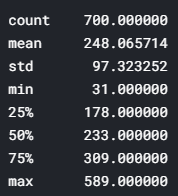
\includegraphics[width=5cm]{./Imagenes/Modelo/estadistica.png}
		\centering 
		\caption{Estadísticas de las palabras}
	\end{figure}
	Lo que podemos observar en la imagen anterior es:
	\begin{itemize}
		\item Count: el cual es el número de canciones analizadas.
		\item Mean: el promedio de palabras por canción.
		\item Std: la desviación estándar de las palabras.
		\item Min: la menor cantidad de palabras encontradas en una canción.
		\item Max: la mayor cantidad de palabras encontradas en una canción.
	\end{itemize}
	Además, se le realizo una tokenizacion a las letras de nuestras 700 canciones, esto quiere decir que se separo cada palabra y cada palabra se convirtió en un número. Para este proceso se hizo uso de Keras y la clase Tokenizer(), la cual cuenta con dos métodos importantes:
	\begin{itemize}
		\item \_fit\_ontext(): El cual actualiza el vocabulario interno en función de una lista de textos determinada o, en este caso, la columna "Lyrics", donde cada entrada de la lista será un token.
		\item \_texts\_tosequences(): El cual transforma cada texto dentro de la lista de textos proporcionados en una secuencia de números enteros; solo se considerarán las palabras conocidas por el tokenizador.
	\end{itemize}	
	\begin{figure}[H]
		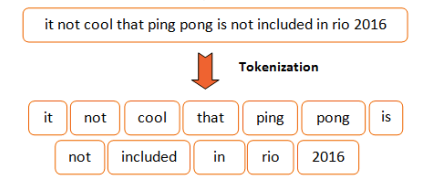
\includegraphics[width=10cm]{./Imagenes/Modelo/tokenization.png}
		\centering 
		\caption{Tokenizado de las palabras \cite{tokenimagen}}
	\end{figure}
	Antes de la generación del modelo, es necesario normalizar todas las oraciones a una misma longitud estándar, para evitar el desbordamiento de la memoria y conseguir que las capas del modelo sean mucho más profundas, este es un proceso simple el cual consta de agregar ceros al comienzo del texto, dando como resultado capas del mismo tamaño.\\\\
	La posición donde se sumarán los ceros viene determinada por el relleno del argumento, en este caso, se hará al comienzo de la secuencia.
	\begin{figure}[H]
		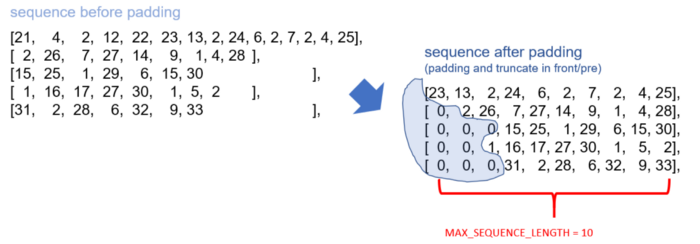
\includegraphics[width=10cm]{./Imagenes/Modelo/padding.png}
		\centering 
		\caption{Padding del tokenizado de las palabras}
	\end{figure}	
	\newpage	
	\section{Creación del modelo}
	En este caso se utilizó el modelo LSTM Bidireccional, este tipo de redes neuronales se ejecutan como su nombre lo indica: en dos direcciones. Esto quiere decir que va del pasado al futuro y viceversa, así es como el modelo conserva la información de ambos estados en cualquier momento. Las redes neuronales de LSTM se utilizan principalmente cuando el contexto está involucrado.\\\\
	Los modelos en Keras se definen como una secuencia de capas, y el modelo secuencial se trata de agregar capas de una en una. Las capas son el componente básico de la red neuronal.\\\\
	Dentro de estas capas podemos encontrar:
	\subsection{Embedding o incrustación}
	Es una capa central, solo se puede usar como la primera capa en un modelo, convierte los números enteros positivos en vectores densos de un tamaño fijo (el primer parámetro es el tamaño del vocabulario, el segundo parámetro es la dimensión de la incrustación densa y el tercer parámetro es sobre la longitud de las secuencias, este se requiere ya que usaremos una capa densa más adelante)
	\begin{center}
		\lstinputlisting[language=Python]{./Imagenes/Modelo/embedding.py}
	\end{center}
	\subsection{Bidireccional}
	Es una capa recurrente, una envoltura bidireccional para las redes neuronales de tipo RNN's que recibirá una capa como entrada, siendo la capa LSTM la que elegimos, recibirá un entero positivo como entrada que se refiere a la cantidad de nodos de salida que se deben devolver.
	\begin{center}
		\lstinputlisting[language=Python]{./Imagenes/Modelo/bidireccional.py}
	\end{center}
	\subsection{Dropout}
	Es una capa de regularización. Esta capa establece aleatoriamente las unidades de entrada en 0, con una frecuencia del valor que le pasamos, en cada paso durante el tiempo de entrenamiento, lo que ayuda a evitar el sobreajuste.
	\begin{center}
		\lstinputlisting[language=Python]{./Imagenes/Modelo/dropout.py}
	\end{center}
	\subsection{Densidad}
	Es una capa central y una capa de red neuronal densamente conectada. Recibe como primer parámetro un entero positivo que se refiere a la cantidad de nodos de salida que deben devolverse. El segundo parámetro es el llamado activación que define el tipo de predicciones que puede hacer el modelo; para el tipo de problema que estamos considerando, el que se adapta mejor es softmax, que genera un vector de valores (entrada) que puede interpretarse como probabilidades de ser utilizado.
	\begin{center}
		\lstinputlisting[language=Python]{./Imagenes/Modelo/dense.py}
	\end{center}
	\subsection{Método de compilación, algoritmo de optimización y métrica de rendimiento}
	Perdida: También conocida como función de costos; funciona durante el proceso de optimización y su función es calcular el error del modelo. La entropía cruzada se utiliza para estimar la diferencia entre una distribución de probabilidad estimada y predicha. Se utilizará categorical\_cross-entropy porque es más adecuado para este tipo de problemas y se usa casi universalmente para entrenar redes neuronales de aprendizaje profundo debido a los resultados que produce.
	Optimización: Se encarga de reducir las pérdidas y brindar los resultados más precisos posibles. Adam es la opción elegida porque es la mejor opción que ofrece Keras para entrenar la red neuronal en menos tiempo y de manera más eficiente. Earlystop detendrá el entrenamiento si el modelo ha dejado de mejorar, esto se verificará al final de cada epoch. En este caso, la "precisión" o “accuracy” se utilizará como métrica de rendimiento.
	El método fit es el encargado de entrenar el modelo para el número fijo de epochs dados.	
	\begin{center}
		\lstinputlisting[language=Python]{./Imagenes/Modelo/compile.py}
	\end{center}
	Quedando como resultado el código del modelo de la siguiente forma:
	\begin{center}
		\lstinputlisting[language=Python]{./Imagenes/Modelo/modelo.py}
	\end{center}
	\subsection{Importación del modelo}
	Una vez completado el entrenamiento de nuestro modelo, lo que falta es importarlo para probar cómo funciona, en nuestro caso nombramos al modelo “song\_lyrics\_generator” y se importo de la siguiente forma, llamándola link de nuestra libreta de Kaggle:
	\begin{center}
		\lstinputlisting[language=Python]{./Imagenes/Modelo/import.py}
	\end{center}
	Ya que contemos con el modelo importado, se creó una función que se utilizará para generar la letra de una canción utilizando el modelo previamente entrenado, predecirá las siguientes palabras en base a la palabra(s) de entrada suministradas como 'seed\_text'. Para que esto funcione, se debe aplicar una tokenización al seed\_text, luego se aplicará un relleno a las secuencias generadas y se pasará al modelo entrenado para que se pueda predecir la siguiente palabra.
	\begin{center}
		\lstinputlisting[language=Python]{./Imagenes/Modelo/function.py}
	\end{center}	
	\newpage
	\section{Desarrollo de la aplicación web}
	Para el desarrollo de la aplicación web se decidió realizarla haciendo uso de React o mejor conocida como ReactJS la cual se trata de una biblioteca de Java para crear interfaces interactivas, con la cual se puedes diseñar vistas simples y en las cuales se actualizarán y renderizarán los componentes necesarios cuando haya cambios en los datos.\\\\
	Se decidió usar este, debido a que nos da la posibilidad de que sea compatible con dispositivos móviles sin la necesidad de volver a escribir código para esta tecnología.\\\\
	Lo primero que se requirió para poder trabajar con React fue descargar Node.js desde su página (https://nodejs.org/es/) la cual nos va a permitir crear aplicaciones web utilizando JavaScript, además de que al instalarlo obtendremos npm el cual posteriormente nos permitirá instalar paquetes con los que añadiremos nuevas funciones a nuestra aplicación y que a su vez son compatibles con React.\\\\
	Una vez que se tiene instalado Node.js para poder ejecutar una aplicación web, en terminal tendremos que escribir npm start, lo cual ejecutara un servidor de desarrollo de manera local, a la cual se puede acceder a través de la siguiente dirección (localhost:3000) en cualquier navegador.\\\\
	Como React se basa en crear vistas lo primero que se hizo fue visualizar que es lo que queremos que vea el usuario, por ello se creó una carpeta en la cual se colocaron las páginas con las cuales se iban a trabajar y con las que el usuario va a interactuar. Estas fueron la página de inicio, la de preguntas frecuentes, la de ejemplos de canciones previamente generadas y una acerca de nosotros.\\\\
	\begin{figure}[H]
		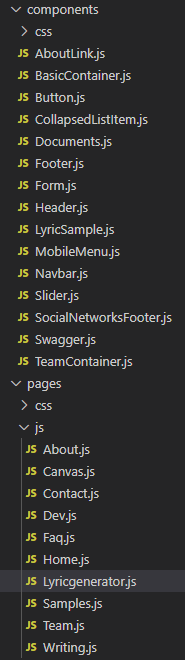
\includegraphics[width=5cm]{./Imagenes/AplicacionWeb/Paginas.png}
		\centering 
		\caption{Páginas trabajadas}
	\end{figure}
	La más importante de estas páginas es la página principal, debido a que es esta la primer a que va a ver el usuario y con la que más va a interactuar, en esta, aparece un mensaje con un botón el cual invita al usuario a generar su propia letra musical.
	\begin{figure}[H]
		\includegraphics[width=13.5cm]{./Imagenes/AplicacionWeb/Paginaweb.png}
		\centering 
		\caption{Página de bienvenida}
	\end{figure}
	Si el usuario le da clic al botón, como React usa estados para renderizar lo que ve el usuario, se muestra en pantalla el formulario donde se le pide al usuario que introduzca una palabra en el idioma inglés, así como se muestra una barra donde el usuario puede ingresar que tanto quiere que rime la letra de esta canción.
	\begin{figure}[H]
		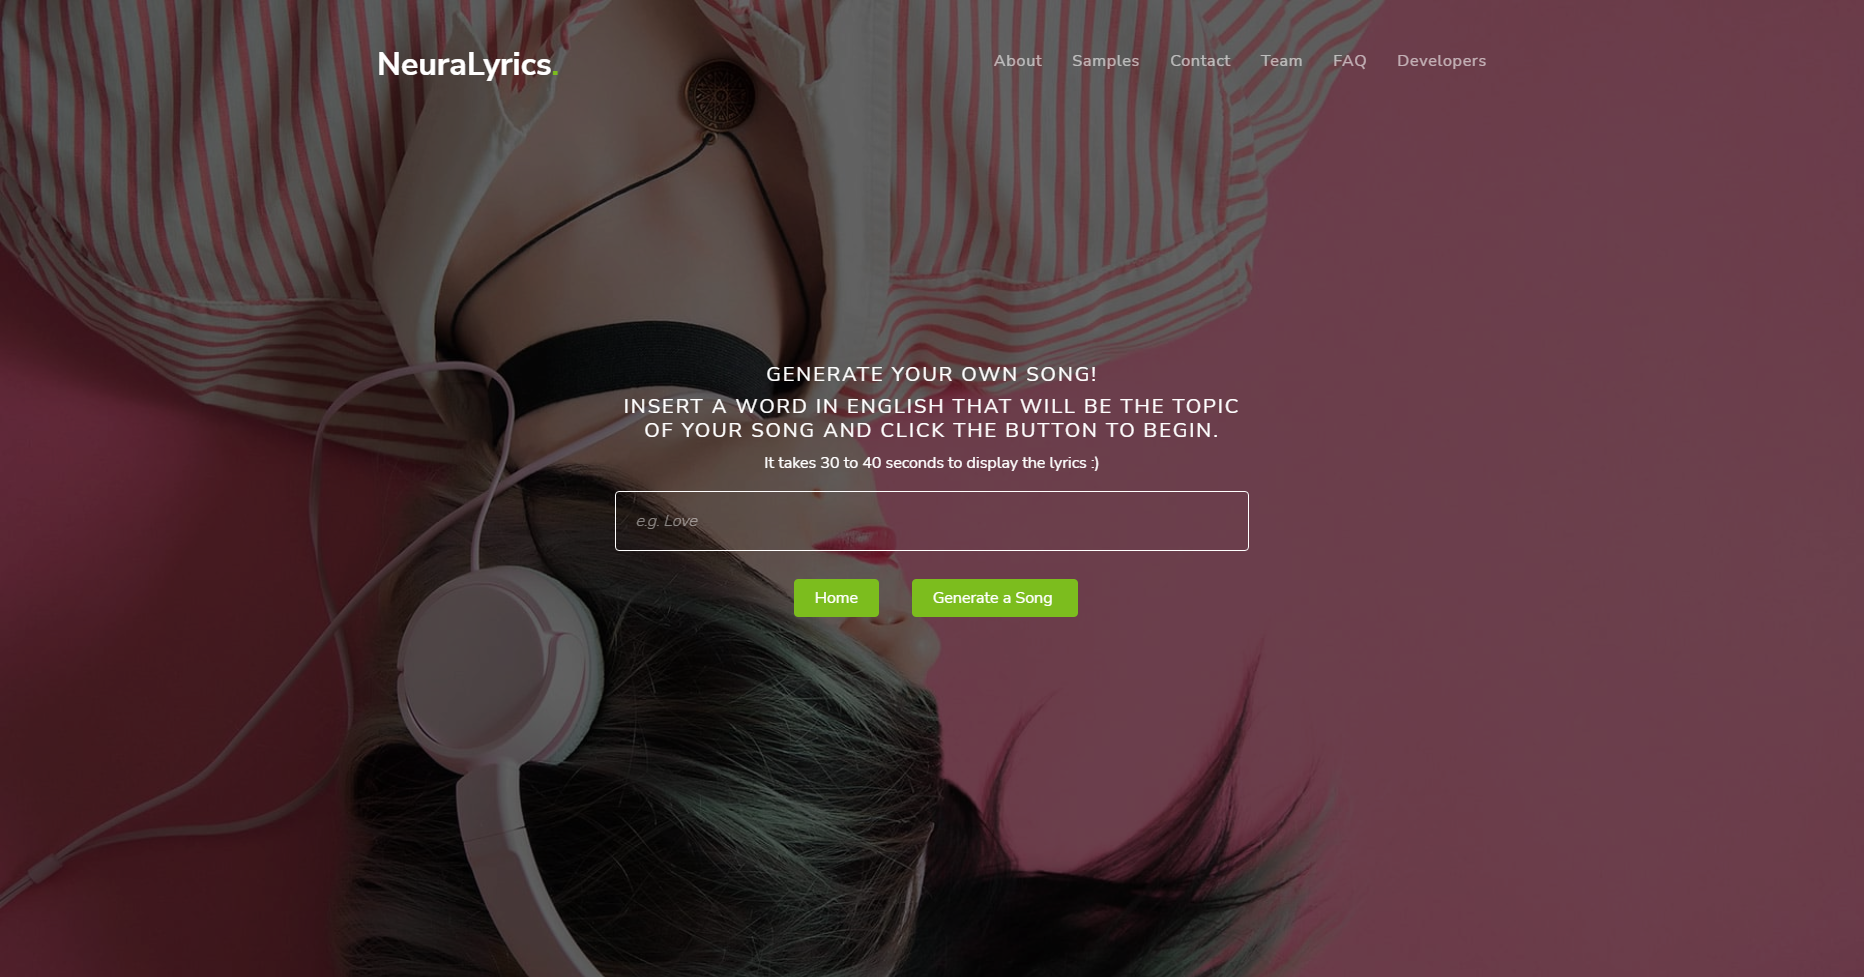
\includegraphics[width=13.5cm]{./Imagenes/AplicacionWeb/pform.png}
		\centering 
		\caption{Formulario}
	\end{figure}
	En esta parte debemos detenernos para habar acerca de cómo es que los datos proporcionados por el usuario son leídos y posteriormente enviados a nuestro back-end para ser procesados futuramente por el modelo. A continuación, se muestra el código de la función la cual realiza este proceso.
	\begin{center}
		\lstinputlisting[language=JavaScript]{./Imagenes/AplicacionWeb/Sendword.js}
	\end{center}
	En esta función lo primero que se hace es recibir los datos (la palabra y el porcentaje) que introdujo el usuario, esto se hace buscado los identificadores de los elemento de la página y obteniendo sus valores, estos, se enviaran al back-end usando la función de fetch, lo que hace dicha función es buscar la url, que en este caso es donde se encuentra alojado nuestro back-end y busca el método post de esta, como el método post de nuestro back-end recibe datos en formato json, los datos que introdujo el usuario deben ser enviados en este formato.\\\\
	Una vez que el usuario le dio clic al botón de generar canción se muestra una leyenda la cual le pide al usuario que aguarde unos segundos, que se está trabajando en su letra. Pasados unos segundos después, en pantalla se le mostrara la letra de la canción generada, así como 3 botones, el primero de ellos le permite descargar la letra generada en un archivo de texto, el segundo le permite al usuario generar una nueva canción utilizando los mismos parámetros con los que genero la letra actual y el ultimo lo regresa al estado anterior para introducir nuevos parámetros y con estos generar una nueva letra.
	\begin{figure}[H]
		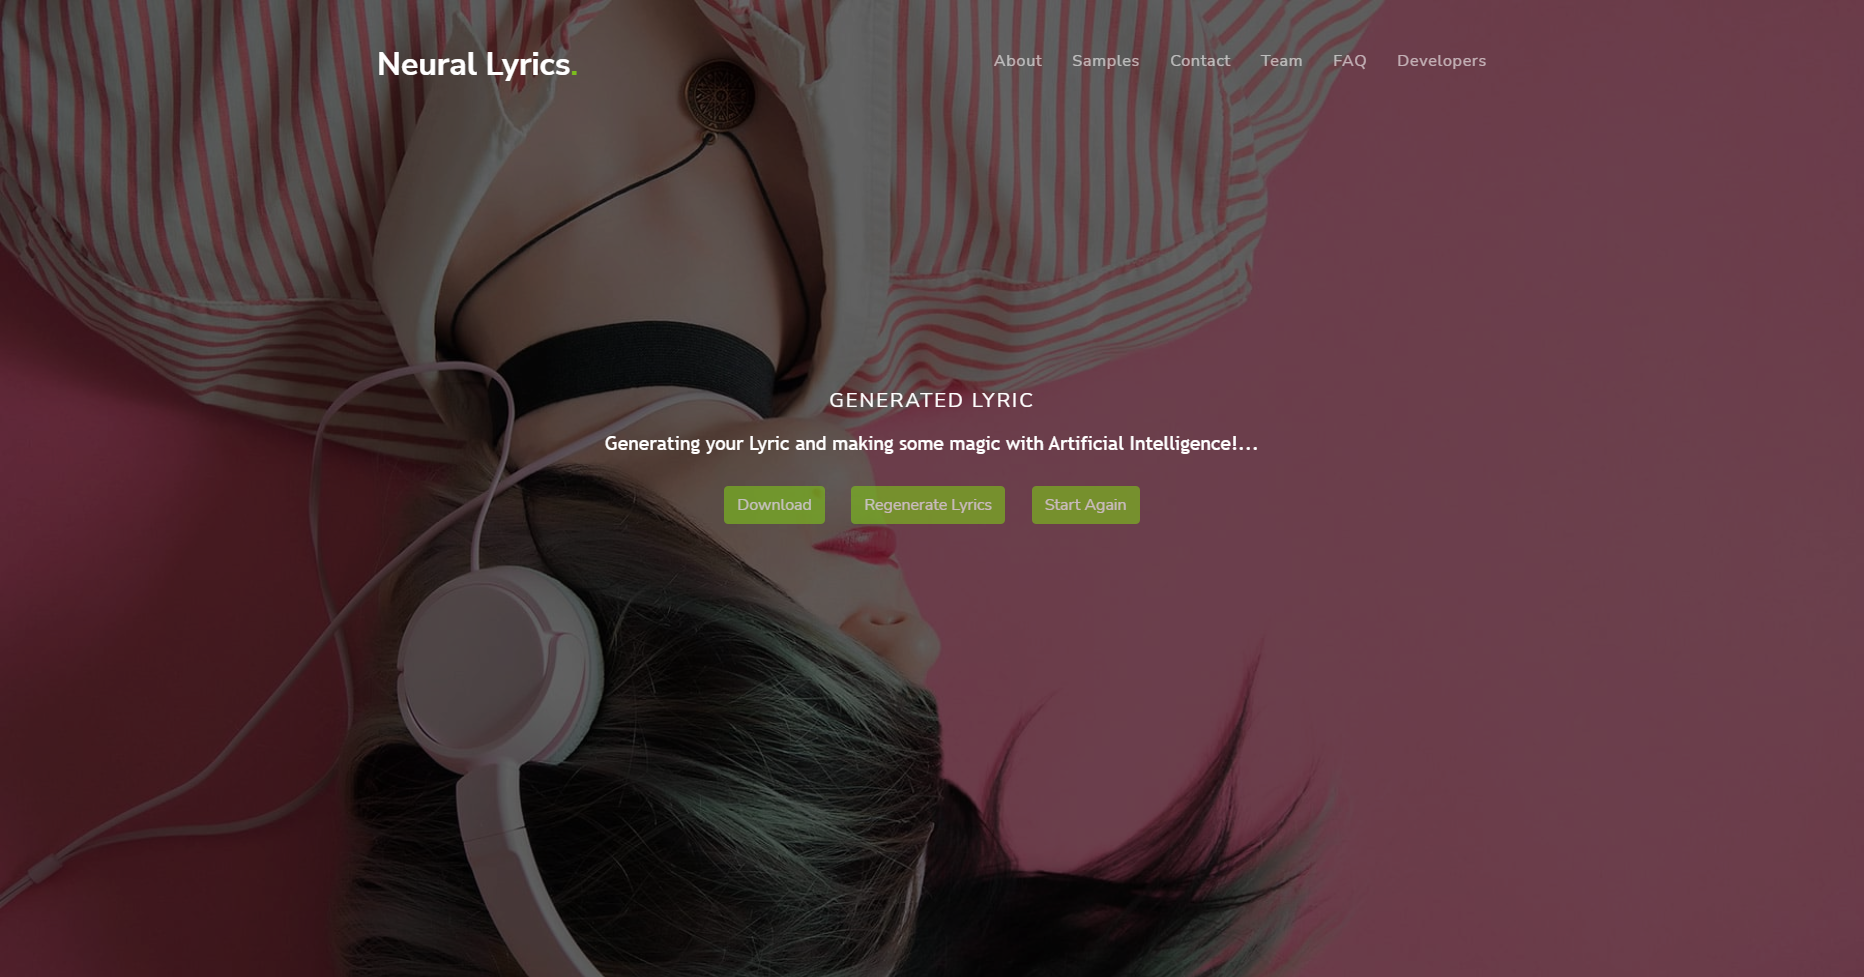
\includegraphics[width=13.5cm]{./Imagenes/AplicacionWeb/pgenerating.png}
		\centering 
		\caption{Leyenda mostrada}
	\end{figure}
	\begin{figure}[H]
	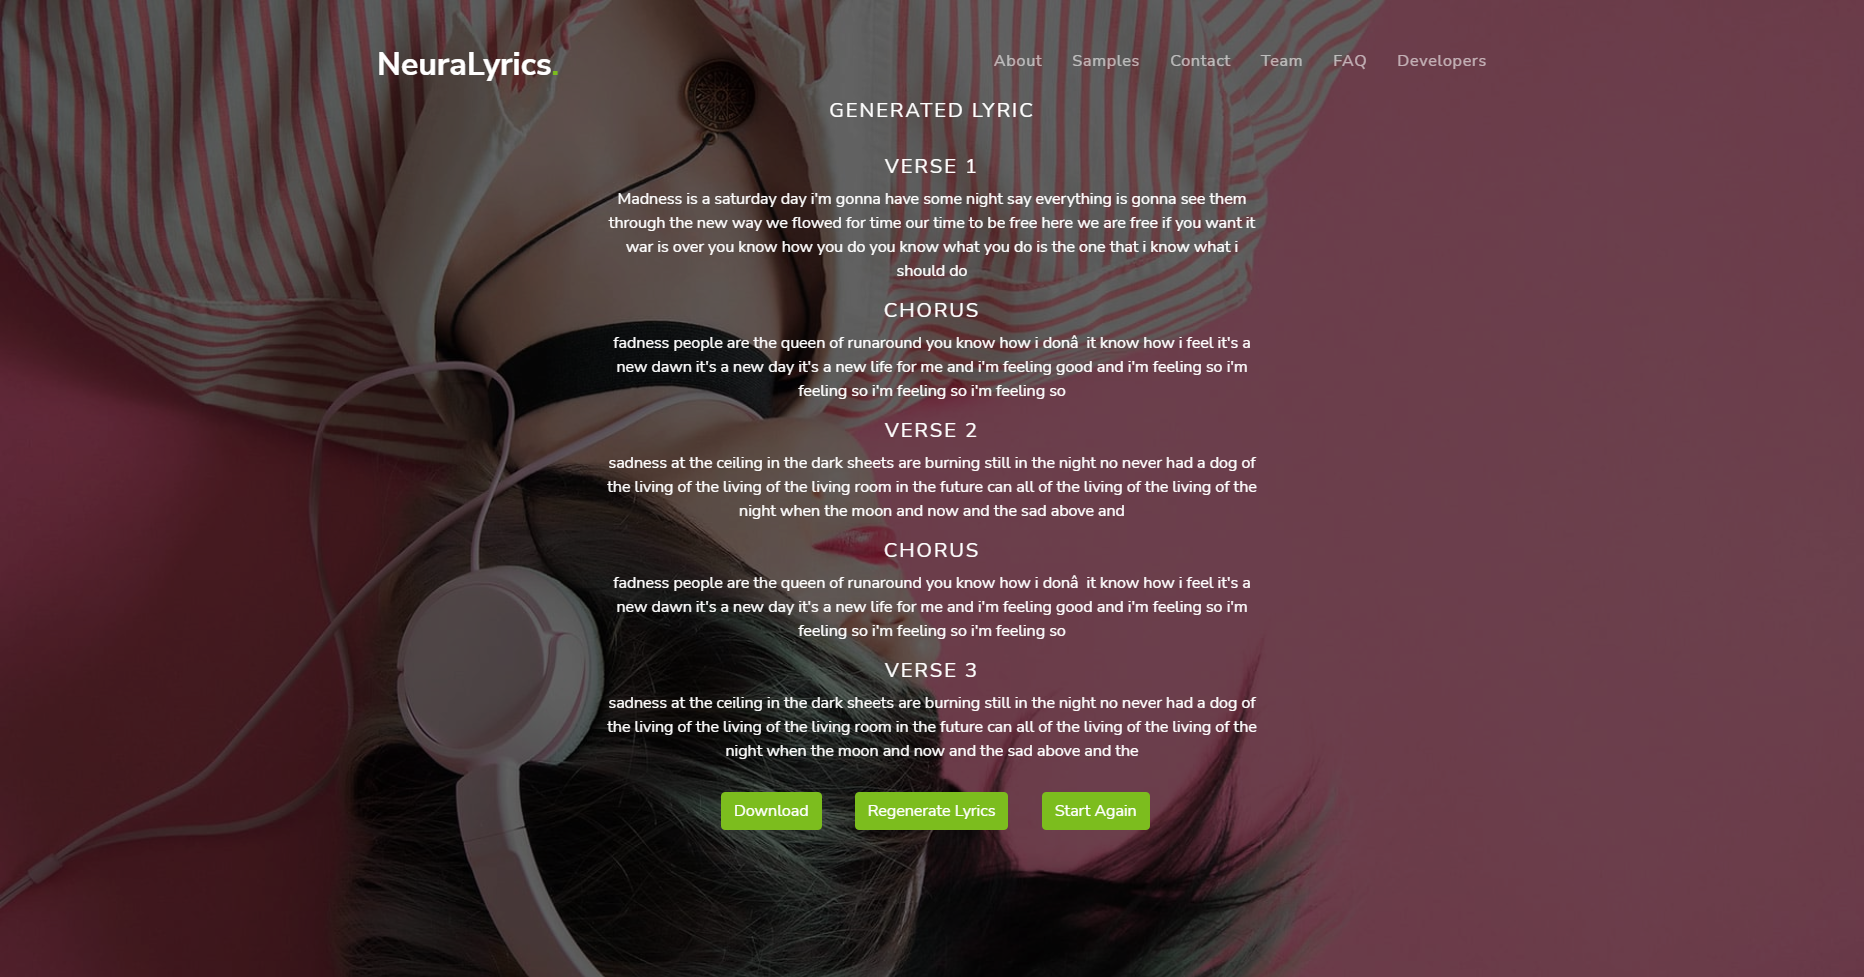
\includegraphics[width=13.5cm]{./Imagenes/AplicacionWeb/Generated.png}
	\centering 
	\caption{Texto generado}
	\end{figure}
	Adentrándonos a esta sección, la primera función que debemos revisar es la que permite hacer la conexión con el back-end para que la página pueda recibir el texto generado por el modelo.
	\newpage
	\begin{center}
		\lstinputlisting[language=JavaScript]{./Imagenes/AplicacionWeb/ModelConection.js}
	\end{center}
	Lo que se hace en el código anterior es realizar una conexión asíncrona con el back-end, esto para que mientras no se reciba una respuesta el usuario en pantalla vea una leyenda que diga que se está trabajando en su texto, cuando en la conexión se reciba una respuesta la leyenda que ve el usuario cambiara, mostrando el texto recibido en la función.
	\begin{center}
		\lstinputlisting[language=JavaScript]{./Imagenes/AplicacionWeb/Download.js}
	\end{center}
	Con esta función se permite crear un archivo de texto el cual es posible descargarse en la computadora del usuario y el cual va a contener la letra de la canción que se generó en ese momento.
	\begin{figure}[H]
		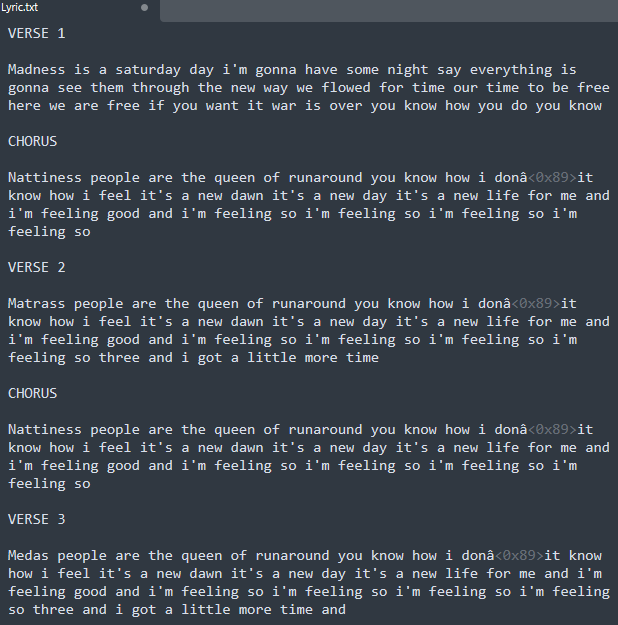
\includegraphics[width=10cm]{./Imagenes/AplicacionWeb/Archivo.png}
		\centering 
		\caption{Archivo de texto descargado}
	\end{figure}	
	Para el segundo botón se utiliza la misma función que se ve en la vista previa se reenvía al back-end los parámetros utilizados y se renderiza nuevamente la vista con la leyenda de que espere unos segundos. En el caso del tercer botón solo se activa el estado que permite renderizar la parte donde el usuario introduce los datos.
	\newpage
	\section{Desarrollo del back-end}
	Para el back-end se decidió trabajar con una aplicación web desarrollada en Flask, debido a que de esta manera era fácil y rápida de implementar, además que permitía una mejor integración con el modelo y la aplicación web previamente trabajada en React.\\\\
	Para poder trabajar con una aplicación web en Flask lo primero que se tiene que hacer o que se recomienda hacer es crear un ambiente virtual usando virtualenv esto para separar nuestro Python instalado originalmente en la computadora del que se va a utilizar en la aplicación. Una vez realizado esto, se inició el desarrollo del código.
	\begin{center}
		\lstinputlisting[language=Python]{./Imagenes/BackEnd/app.py}
	\end{center}
	En el código app.py mostrado anteriormente es el código principal de nuestro back-end ya que es este el que se despliega en el navegador web, en este lo primero que se visualiza al entrar es información con respecto a esta aplicación como su nombre, versión y los plugins con los que esta cuenta.\\\\
	Para poder ver un cómo es que realmente funciona el back-end se realizó una pequeña interfaz y es posible acceder a ella a través de la siguiente dirección x/swagger-ui/ en ella podemos encontrar con mayor detalle el status actual de la api, la cual se encuentra ubicada en el espacio nombrado como health.
	\begin{figure}[H]
		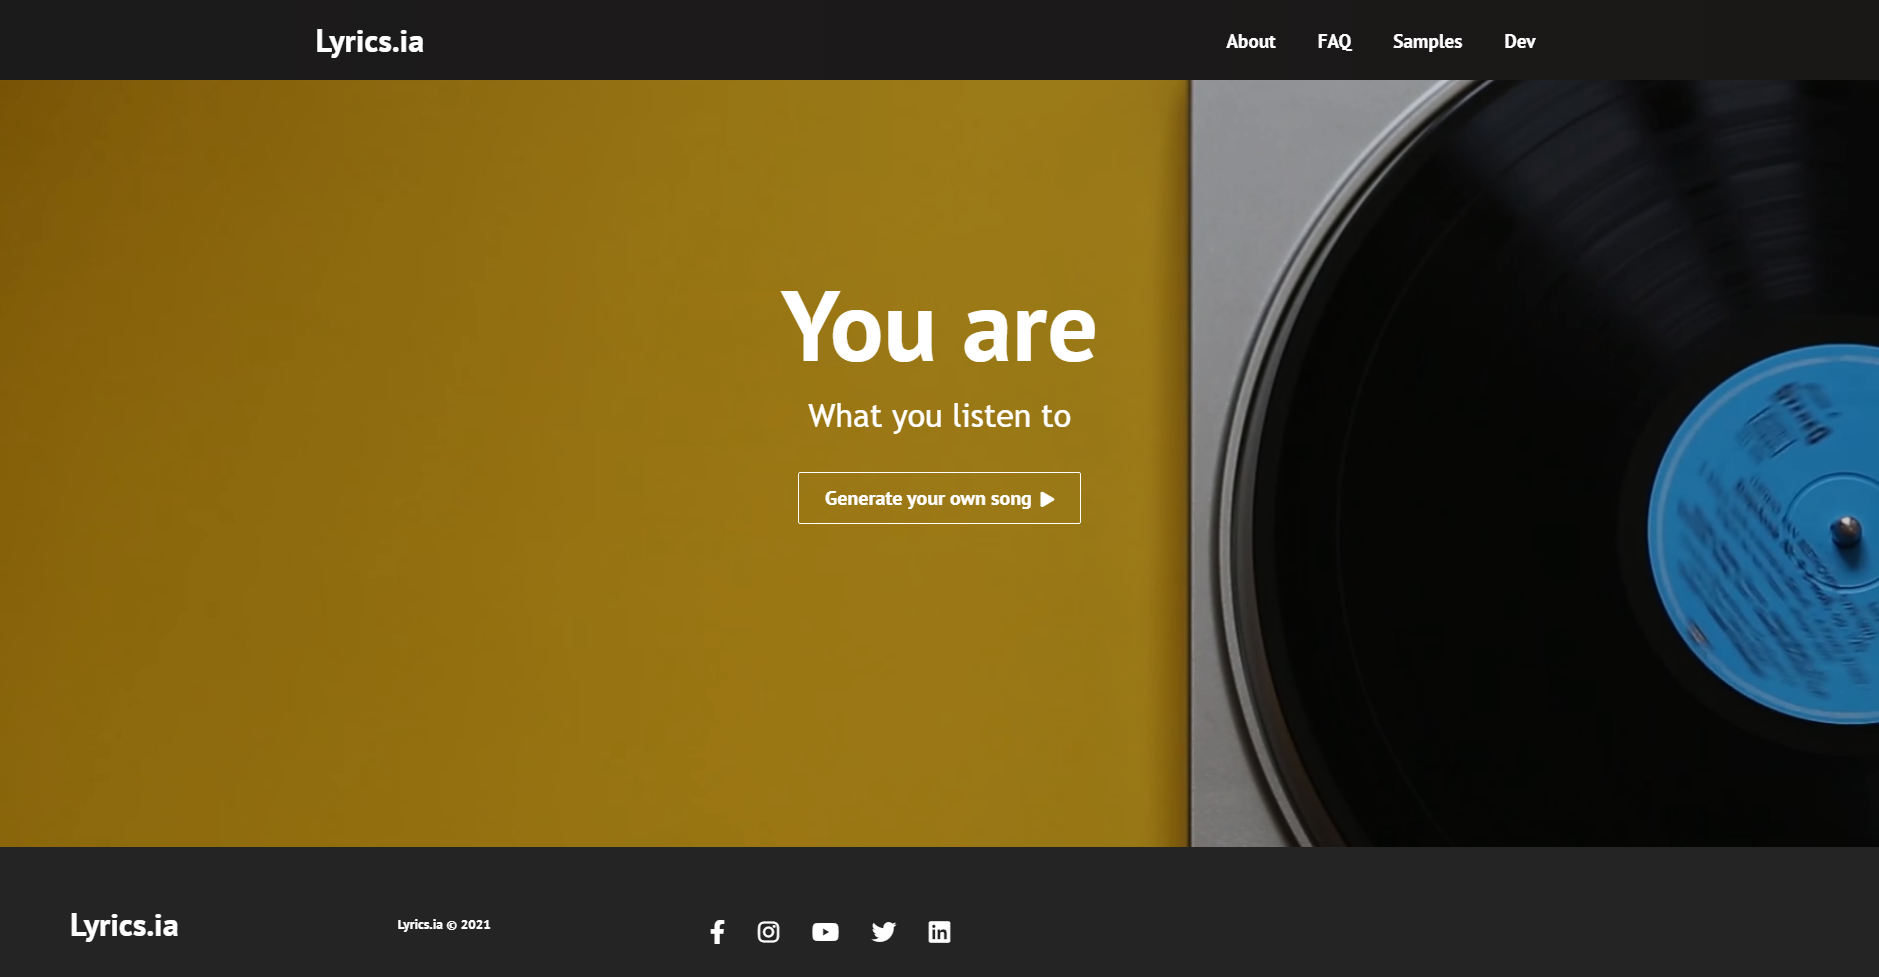
\includegraphics[width=13.5cm]{./Imagenes/BackEnd/Health.png}
		\centering 
		\caption{Cuadro de status del Back-end}
	\end{figure}
	Un poco más abajo se encuentra el método post de la api, este es el encargado de recibir la información de la aplicación web realizada en React en formato json, para posteriormente enviar esta información al modelo
	\begin{figure}[H]
		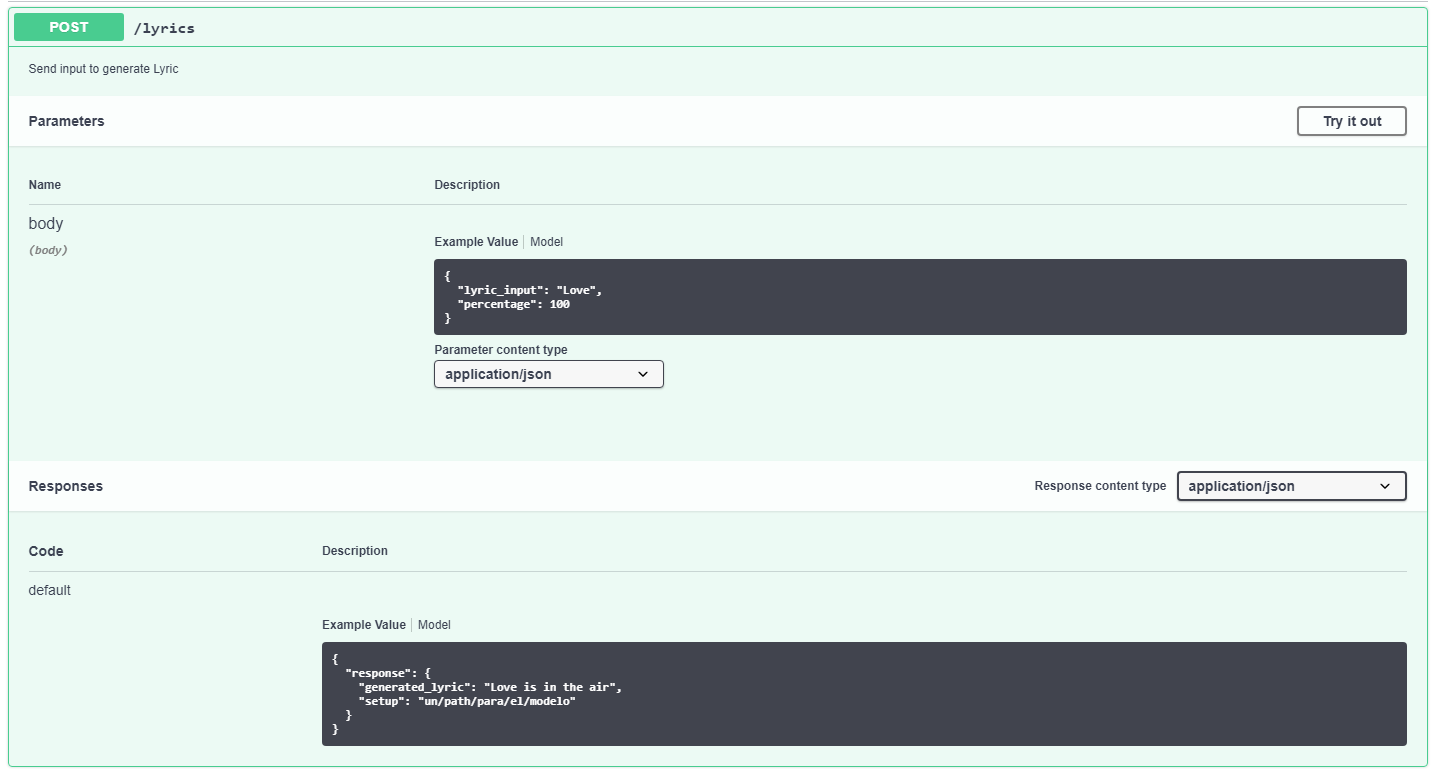
\includegraphics[width=13.5cm]{./Imagenes/BackEnd/Post.png}
		\centering 
		\caption{Cuadro del método Post}
	\end{figure}
	Para realizar esta tarea se desarrolló el siguiente código
	\begin{center}
		\lstinputlisting[language=Python]{./Imagenes/BackEnd/generate_lyrics.py}
	\end{center}
	En este código utilizando la palabra y el porcentaje introducidos por el usuario son enviados al modelo para ser procesados generando así un texto, este procedimiento se realiza en la función generate\_lyric, e; texto generado va a ser regresado a nuestra api para mandarlo a la aplicación web en React para posteriormente mostrarla en el navegador web del usuario.
	\newpage
	\section{Desplegando componentes}
	
	\subsection{Despliegue del back-end}
	
	\subsection{Despliegue de la página web}
	
	Para el despliegue de la pagina web nos apoyamos de la plataforma Vercel, la cual permite que los desarrolladores puedan desplegar sus paginas de manera rápida, así como poder actualizarla y escalarla de manera sencilla, además permite hacer despliegues de proyectos que se encuentran dentro de una cuenta de Github\\\\
	Lo primero que debemos hacer para poder trabajar con la línea de comandos de Vercel es instalarlo, para ello debemos recurrir a nuestra terminal e instarlo usando el comando npm i -g vercel o yarn global add vercel.
	\begin{figure}[H]
		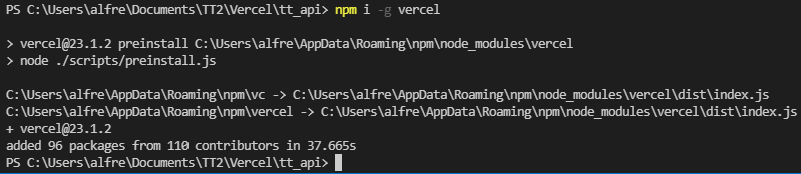
\includegraphics[width=12cm]{./Imagenes/Despliegue/Instalacion.png}
		\centering 
		\caption{Instalando CLI de Vercel}
	\end{figure}
	Una vez instalado, debemos abrir la carpeta de nuestro proyecto a desplegar, y en una terminal dentro de esa carpeta solo es necesario escribir vercel para abrir el CLI de Vercel el cual nos preguntara si el proyecto contenido dentro de la carpeta es el que se va a configurar y desplegar, a lo cual damos una respuesta afirmativa, posteriormente nos pide quien lo va a desplegar, para ello usamos una cuenta creada en esta plataforma o vinculamos la de Github para acceder, se nos pregunta el nombre del proyecto y el inicio de los archivos del proyecto a desplegar.
	\begin{figure}[H]
		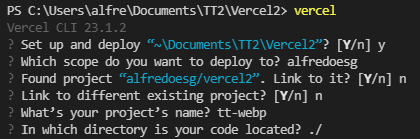
\includegraphics[width=12cm]{./Imagenes/Despliegue/Acciones.png}
		\centering 
		\caption{Indicando acciones para el despliegue}
	\end{figure}
	Después de dar las indicaciones anteriores el CLI de vercel detecta automáticamente el tipo de proyecto trabajado, en este caso una aplicación web usando React, para por último preguntar si se quiere cambiar la configuración del trabajo encontrado, en este caso decimos que no, ya que es correcto el tipo de aplicación encontrada con el trabajado.
	\begin{figure}[H]
		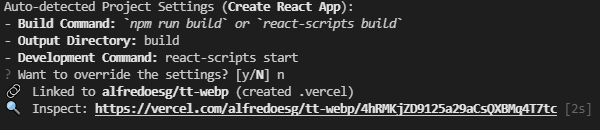
\includegraphics[width=12cm]{./Imagenes/Despliegue/Deteccion.png}
		\centering 
		\caption{Deteccion del tipo de proyecto a desplegar}
	\end{figure}
	Vercel comienza a desplegar la aplicación web y nos da un enlace en el cual podemos ver como se encuentra el despliegue, si se presentara algún problema, en la terminal nos indicara cual es.
	\begin{figure}[H]
		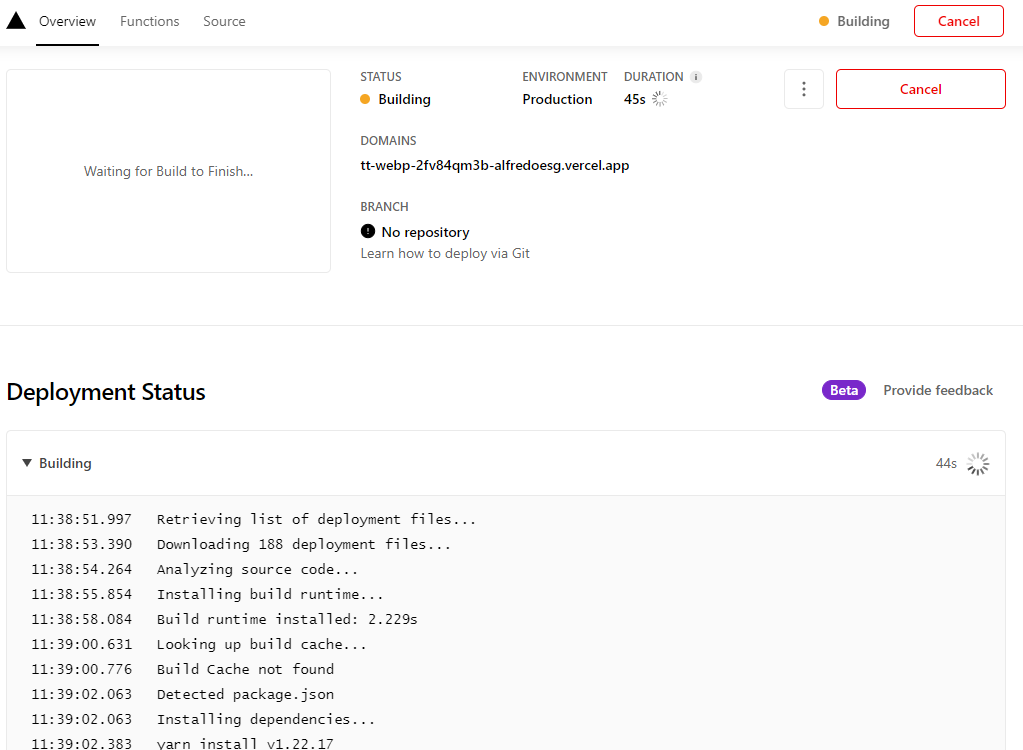
\includegraphics[width=12cm]{./Imagenes/Despliegue/Desplegando.png}
		\centering 
		\caption{Desplegando el proyecto}
	\end{figure}
	Al momento de desplegar la aplicación nos marca un error.
	\begin{figure}[H]
		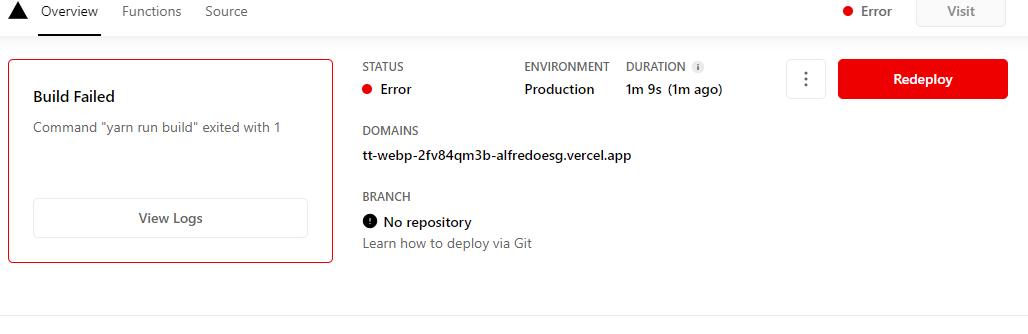
\includegraphics[width=12cm]{./Imagenes/Despliegue/Error.png}
		\centering 
		\caption{Desplegando el proyecto}
	\end{figure}
	Este error está relacionado con unas librerías opcionales localizadas dentro de la careta node\_modules de nuestro proyecto, vercel no reconoce que estas librerías son opcionales, para poder hacer el despliegue y que no nos marque estas librerías opcionales como error debemos entrar a la parte de configuraciones de nuestro proyecto.	
	\begin{figure}[H]
		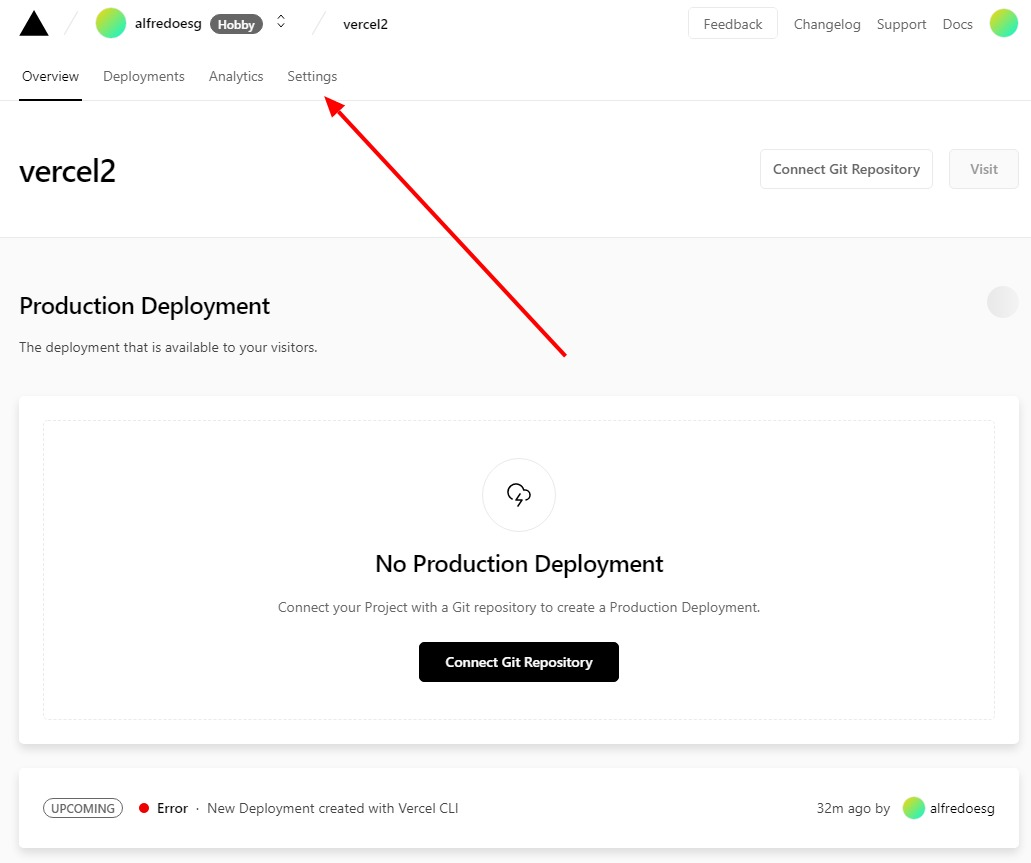
\includegraphics[width=12cm]{./Imagenes/Despliegue/Ajustes.jpeg}
		\centering 
		\caption{Configuración del proyecto desplegado}
	\end{figure}
	Luego en la parte de variables de entorno y en esta sección agregar la variable CI con un valor de false
	\begin{figure}[H]
		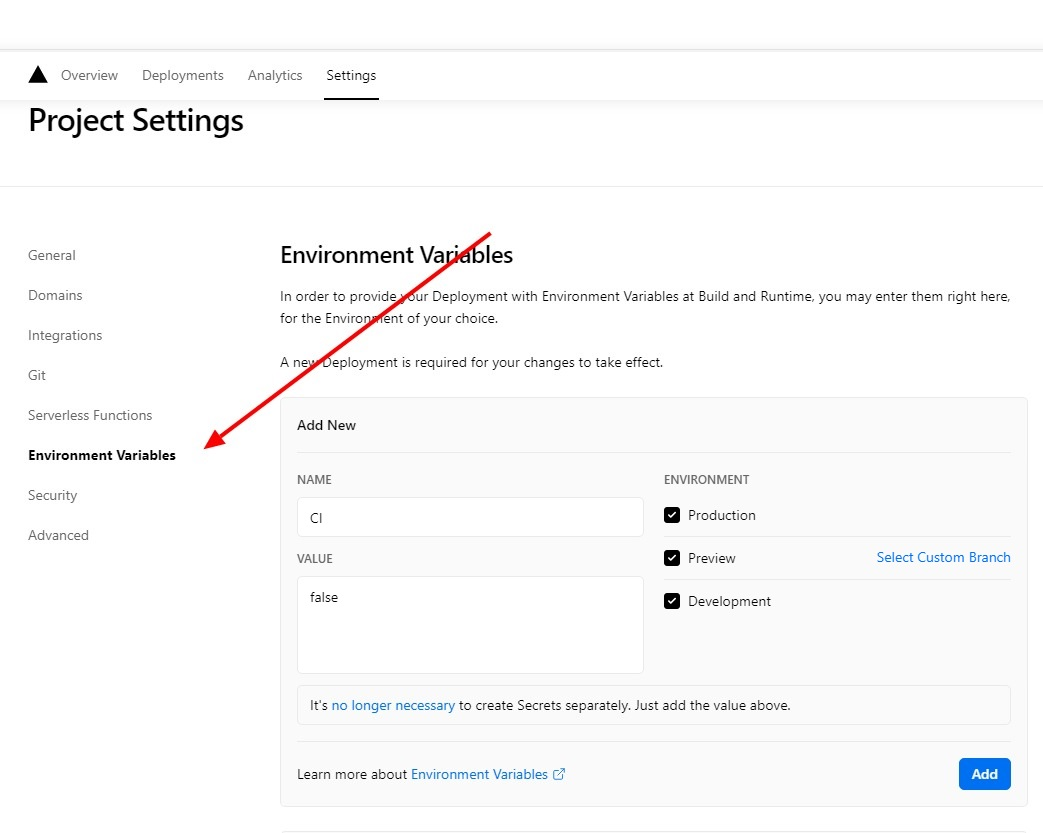
\includegraphics[width=12cm]{./Imagenes/Despliegue/Varaiblesentorno.jpeg}
		\centering 
		\caption{Varaible de entorno}
	\end{figure}
	Después de realizar esto volvemos a nuestra terminal, volvemos a escribir vercel y automáticamente vuelve a realizar el despliegue de la aplicación web, de esta misma forma solo escribiendo vercel en la terminal la actualización de la página desplegada ante algún cambio en el código.\\\\
	Una vez completado el despliegue, se nos genera un enlace con el cual se puede acceder a la aplicación web ya desplegada desde cualquier dispositivo.
	\begin{figure}[H]
		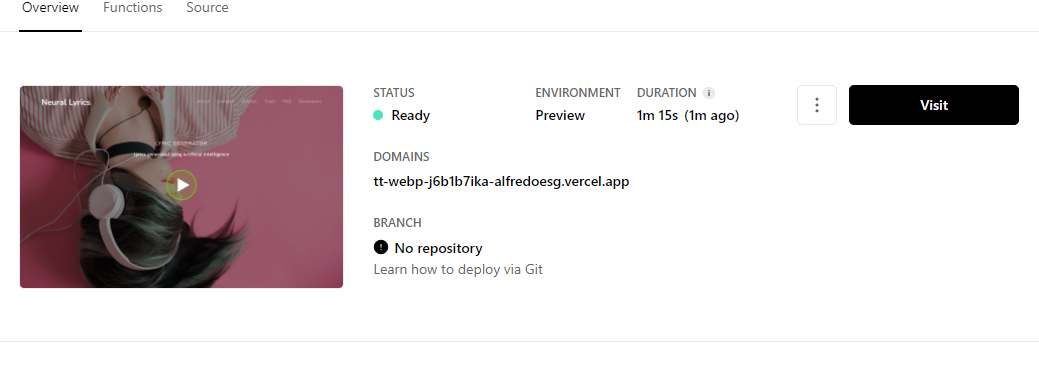
\includegraphics[width=12cm]{./Imagenes/Despliegue/Desplegada.png}
		\centering 
		\caption{Aplicación web desplegada}
	\end{figure}
	\begin{figure}[H]
		\includegraphics[width=12cm]{./Imagenes/Despliegue/Paginaweb.png}
		\centering 
		\caption{Accediendo a la aplicación web desplegada}
	\end{figure}
	En nuestro caso, previamente se había adquirido un dominio, para realizar el cambio del enlace proporcionado por Vercel a el enlace del dominio previamente adquirido, en nuestro proyecto, en la parte de configuración, en la de domino, se agrega el enlace y así es posible acceder a esta pagina web desde ese dominio adquirido.
	\newpage
	\section{Configuración de SSL y DNS}
	
	Para permitir que nuestra pagina web pueda accederse desde otros dispositivos es necesario hacer la configuración correcta de DNS y darle un certificado de seguridad. Debido a que nuestra pagina web fue desplegada en la plataforma de Vercel, para que esta pueda direccionarse de manera correcta con nuestro dominio se requiere la configuración de un DNS especifico que nos pide Vercel.
	\begin{figure}[H] 
		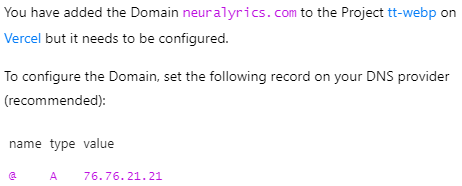
\includegraphics[width=10cm]{./Imagenes/DnsSSL/Dns1.png}
		\centering \caption{Dirección IP requerida para la configuración del DNS.}
	\end{figure}
	\begin{figure}[H] 
		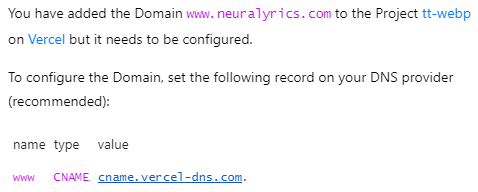
\includegraphics[width=10cm]{./Imagenes/DnsSSL/Dns2.png}
		\centering \caption{Nombre requerido para la configuración del DNS.}
	\end{figure}
	
	Estas reglas de DNS deben agregarse en la plataforma de Cloudflare de la siguiente manera (METELE TEXTO ADRIAN QWQWQWQWQWQWQWQWQWQWQWQWQWQW)
	
	
	En cuanto a la parte de seguridad de nuestra pagina web, como requiere que el usuario introduzca una palabra y esta posteriormente procesarla y mandarla a nuestro back-end, para ello se requirió configurar un certificado SSL para de esta manera tener una seguridad en el manejo de la información entre el servido del front-end y el back-end.\\\\
	Para esta configuración nos apoyamos en Amazon Elastic Beans la cual nos permite darle el certificado que requiere el servidor del back-end siguiendo los siguientes pasos (METELE TEXTO ADRIAN QWQWQWQWQWQWQWQWQWQWQWQWQWQW)
	\newpage
	\begin{thebibliography}{20}
		\bibitem{refQuesPython} 
		Python (2021), What is Python? Executive Summary, [En línea]. Disponible: https://www.python.org/doc/essays/blurb/ [Último acceso: 24 de abril del 2021].
		\bibitem{refHtml}
		Mozilla.org (2021, febrero 19), HTML basics, [En línea]. Disponible: https://developer.mozilla.org/en-US/docs/Learn/Getting\_started\_with\_the\_web/HTML\_basics [Último acceso: 15 de mayo del 2021].
		\bibitem{refHtml2}
		Mozilla.org (2021, mayo 14), HTML5, [En línea]. Disponible: https://developer.mozilla.org/es/docs/Web/Guide/HTML/HTML5 [Último acceso: 15 de mayo del 2021].
		\bibitem{refcss}
		W3C (2016), HTML \& CSS, [En línea]. Disponible: [Último acceso: 15 de mayo del 2021].		
		\bibitem{refjs}
		Mozilla.org (2021, abril 27), What is JavaScript?, [En línea]. Disponible: https://developer.mozilla.org/en-US/docs/Learn/JavaScript/First\_steps/What\_is\_JavaScript [Último acceso: 15 de mayo del 2021].
		\bibitem{amazon_ec2}
		Amazon (2021), Amazon EC2 [En línea]. Disponible: https://aws.amazon.com/es/ec2/?ec2-whats-new.sort-by=item.additionalFields.postDateTime\&ec2-whats-new.sort-order=desc [Último acceso: 1 Junio 2021]		
		\bibitem{amazon_sagemaker}
		Amazon (2021), Amazon SageMaker [En línea]. Disponible: https://aws.amazon.com/es/sagemaker/ [Último acceso: 1 Junio 2021]		
		\bibitem{amazon_s3}
		Amazon (2021), Amazon S3 [En línea]. Disponible: https://aws.amazon.com/es/s3/ [Último acceso: 1 Junio 2021]		
		\bibitem{kaggle}
		Kaggle (2010), How to Use Kaggle [En línea]. Disponible: https://www.kaggle.com/docs/datasets [Último acceso: 25 Mayo 2021]
		\bibitem{kaggleDataset}
		Kaggle (2019, Noviembre 17), Song lyrics from 6 musical genres [En línea]. Disponible: https://www.kaggle.com/neisse/scrapped-lyrics-from-6-genres [Último acceso: 25 Mayo 2021]
		\bibitem{vagalume}
		Vagalume (2002), Vagalume: Music e tudo [En línea]. Disponible: https://www.vagalume.com.br/ [Último acceso: 25 Mayo 2021]		
		\bibitem{data_cleaning}
		Aaron Tay (2021, Abril 23), Data Cleaning Techniques [En línea]. Disponible: https://www.digitalvidya.com/blog/data-cleaning-techniques/ [Último acceso: 30 Mayo 2021]
		\bibitem{tokenimagen}
		B. Lee (2019, Noviembre 17), How to 10x Response Rates on Surveys [En línea]. Disponible: https://bryankmlee3.medium.com/conducting-surveys-with-nlp-d38df4c29e39 [Último acceso: 5 Junio 2021]
		
	\end{thebibliography}	
\end{document}